\documentclass[12pt,a4paper]{article}
\usepackage[T1]{fontenc}
\usepackage[utf8]{inputenc}
\usepackage{lmodern}
\usepackage[a4paper,margin=1in]{geometry}
\usepackage{amsmath,amssymb,amsthm,mathtools,bm}
\usepackage{booktabs,array,tabularx,multirow}
\newcolumntype{Y}{>{\raggedright\arraybackslash}X}
\usepackage{graphicx}
\usepackage{enumitem} 
\usepackage{microtype}
\usepackage{hyperref}
\usepackage{xcolor}
\usepackage{caption}
\hypersetup{colorlinks=true,linkcolor=blue!60!black,citecolor=blue!60!black,urlcolor=blue!60!black,
  pdftitle={Distributional Random Forests: Estimation, Inference, and Distributional Heterogeneity}}
% \setlength{\parindent}{0pt}
% \setlength{\parskip}{5pt}
\setlist[itemize]{topsep=2pt,itemsep=1pt} 
\setlist[enumerate]{topsep=2pt,itemsep=1pt}
\newtheorem{proposition}{Proposition}
\newtheorem{remark}{Remark}
\newtheorem{lemma}{Lemma}
\newcommand{\E}{\mathbb E}
\newcommand{\Pp}{\mathbb P}
\newcommand{\R}{\mathbb R}
\newcommand{\calH}{\mathcal H}
\newcommand{\calP}{\mathcal P}
\newcommand{\MMD}{\operatorname{MMD}}
\newcommand{\Var}{\operatorname{Var}}
\newcommand{\Cov}{\operatorname{Cov}}
\newcommand{\1}{\mathbf 1}
\newcommand{\norm}[1]{\left\lVert#1\right\rVert}
\newcommand{\ip}[2]{\left\langle#1,#2\right\rangle}

\title{\Large \textbf{Distributional Random Forests:}\\
 Estimation, Inference, and Distributional Heterogeneity\\[4pt]
 \large ST6242: Combinatorial Statistics and Machine Learning\\
 \large Final Project Report}
\author{Le Thi Hong Ha}
\date{November 2026}

\begin{document}
\maketitle

\begin{abstract}
Distributional random forests (DRF) use maximum mean discrepancy (MMD) to construct forest partitions sensitive to changes in conditional response distributions. This report reviews the estimator, its reproducing kernel Hilbert space (RKHS) interpretation and consistency theory from \'{C}evid et al.\ (2022), together with the Gaussian limit and half-sampling inference developed by N\"af et al.\ (2023). It then surveys follow-up work, which extends DRF to causal effects, variable importance, functional responses, and survey data, and which corrects one step in the proof of the inference theory. I prove that the balanced population MMD split uniquely identifies a distributional change point even when the conditional means coincide. In root-split simulations, MMD splitting is consistently more accurate than CART on squared responses, while mean-CART does not locate the change and is pulled into the high-variance regime. In complete forests across variance, tail-shape, bimodality, and dependence changes, a random Fourier feature (RFF) approximation to MMD splitting improves three of four targeted functionals but has a larger conditional squared MMD than mean-CART in three of four settings. An exact decomposition of this error explains the discrepancy: RFF--MMD places far less weight on observations from the wrong regime, but this reduction in bias is outweighed by a larger remainder term, and most of that increase is in excess of the noise expected under honest weights. A further experiment with smooth variance transitions shows that the advantage of RFF--MMD for conditional variance disappears as the transition widens. All comparisons use paired Monte Carlo errors. My implementation uses fixed Fourier features and non-honest bootstrap trees, so the inferential guarantees for honest DRF do not apply to it.
\end{abstract}

\section{Introduction}\label{sec:intro}
Let $\mathcal D_n=\{(X_i,Y_i)\}_{i=1}^n$ be an independent and identically distributed sample, where $X_i\in\R^p$ is a covariate vector and $Y_i\in\R^d$ is a possibly multivariate response. The dimension of the covariates is $p$ and the response dimension is $d$. Many statistical analyses begin with the conditional mean $m(x)=\E[Y\mid X=x]$. Conditional laws with identical means can exhibit different variances, tail probabilities, dependence structures, and multimodality. Mean estimation can therefore conceal scientifically important distributional heterogeneity.

The more general estimand is the conditional law $P_x:=\mathcal L(Y\mid X=x)$. A reliable estimate $\widehat P_x$ supports multiple statistical targets through a single fitted model. Examples include marginal conditional quantiles, tail probabilities, the conditional covariance matrix, and comparisons of conditional distributions across groups.

\'{C}evid et al.\ \cite{cevid2022} propose \emph{distributional random forests} (DRF), whose split criterion compares the response distributions in prospective daughter nodes using MMD. The resulting random forest constructs data-adaptive, nonnegative weights and a weighted empirical conditional law. N\"af et al.\ \cite{naf2023} subsequently analyze the asymptotic distribution of this estimator and show how half-sampling can approximate sampling uncertainty.

I extend the analysis to answer two questions: (1) what a single MMD split identifies at the population level, and (2) whether distribution-sensitive partitions translate into more accurate conditional laws after forest aggregation. I first reconstruct the DRF algorithm and its RKHS interpretation, then review the consistency and inference theorems together with their assumptions and related work. I then prove a population change-point result, evaluate the root-splitting mechanism, and study complete forests on four step-change designs and on a family of smooth variance transitions.

The survey of follow-up work in Section~\ref{sec:related} finds that later papers mainly broaden the scope of DRF, to causal contrasts, variable importance, function-valued responses, and complex surveys. One of them also corrects a step in the proof of the Gaussian limit of N\"af et al.\ by adding a strengthened honesty assumption. A recent empirical comparison of splitting criteria reaches conclusions consistent with the experiments reported here.

The population calculation identifies a change point between distinct conditional laws even when the conditional mean is constant. In the root-split experiment, MMD is consistently more accurate than CART on squared responses, and both are far more accurate than CART on the original response. In complete forests, RFF--MMD improves three selected distributional functionals, while mean-CART has lower conditional squared MMD in three of four settings. I resolve this apparent contradiction with an exact bias--remainder decomposition of the conditional MMD risk. Distribution-sensitive splitting sharply reduces the weight placed on the wrong regime. Its remainder term, however, grows by more than the bias falls, and most of that growth is attributable to using the same responses to choose splits and to populate leaves. This points to the honesty condition in the assigned papers' theory as the key missing ingredient. The experiment code, per-replication records, paired contrasts, and figure scripts are available at \url{https://github.com/USERNAME/drf-experiments}; % TODO: replace with the actual repository URL
all simulation tables and figures are generated from the saved records. The implementation is independent of the authors' official DRF package.

\section{Background: Forest Weights, Kernels, and MMD}\label{sec:background}
\subsection{From regression forests to conditional distributions}
A regression tree partitions the covariate space and predicts a query point $x\in\R^p$ by averaging training responses in the terminal leaf containing $x$. Consider a forest with $B\ge1$ trees, indexed by $b=1,\ldots,B$. Let $L_b(x)\subseteq\R^p$ denote the terminal-leaf region containing $x$ in tree $b$. Its training observations have indices $\{i:X_i\in L_b(x)\}$. The tree-specific weights $w_{bi}(x)$ and their forest averages are
\begin{equation}\label{eq:treeweights}
 w_{bi}(x)=\frac{\1\{X_i\in L_b(x)\}}{|\{j:X_j\in L_b(x)\}|},\qquad
 \widehat w_{i,B}(x)=\frac{1}{B}\sum_{b=1}^{B}w_{bi}(x).
\end{equation}
For simplicity, \eqref{eq:treeweights} uses the full relevant estimation sample; subsampled or honest trees average over their designated estimation observations. The finite-forest weights $\widehat w_{i,B}(x)$ are nonnegative and sum to one whenever all prediction leaves are nonempty. Let $\mathcal T$ denote the random subsampling and tree-building procedure, and write $w_{\mathcal T,i}(x)$ for the corresponding tree weight. Its conditional expectation defines the \emph{infinite-forest} weight:
\[
 \widehat w_i(x)=\E_{\mathcal T}[w_{\mathcal T,i}(x)\mid\mathcal D_n],
 \qquad \widehat w_{i,B}(x)\longrightarrow\widehat w_i(x)
 \quad\text{as }B\to\infty,
\]
when trees are sampled independently conditional on $\mathcal D_n$. The asymptotic results reviewed in Section~\ref{sec:method} concern this idealized infinite forest. Its estimated conditional kernel mean embedding $\widehat\mu_n(x)$ is defined in \eqref{eq:cme} below.

The infinite-forest prediction is $\widehat m(x)=\sum_i\widehat w_i(x)Y_i$. The same weights define a probability measure
\begin{equation}\label{eq:weightedlaw}
 \widehat P_x=\sum_{i=1}^n\widehat w_i(x)\delta_{Y_i},
\end{equation}
where $\delta_y$ is the Dirac measure at $y$, satisfying $\delta_y(A)=\1\{y\in A\}$ for any measurable event $A$. Thus $\widehat P_x(A)=\sum_i\widehat w_i(x)\1\{Y_i\in A\}$. Its finite-forest counterpart $\widehat P_{x,B}$ uses $\widehat w_{i,B}(x)$ in the same formula. This weighted-distribution viewpoint underlies quantile regression forests \cite{meinshausen2006}. DRF learns \emph{tree partitions sensitive to changes in whole distributions} through MMD-based splitting \cite{cevid2022}.

For scalar responses and any threshold $t\in\R$, the estimated conditional cumulative distribution function is $\widehat F_x(t)=\sum_i\widehat w_i(x)\1\{Y_i\le t\}$. For a quantile level $\tau\in(0,1)$, the estimated conditional quantile is $\widehat q_\tau(x)=\inf\{t:\widehat F_x(t)\ge\tau\}$. For vector responses, the same empirical law permits plug-in estimates of distributional functionals whenever these are well defined.

\subsection{Kernel mean embeddings and maximum mean discrepancy}
Let $k:\R^d\times\R^d\to\R$ be a positive-definite kernel with associated reproducing kernel Hilbert space (RKHS) $\calH$. Its canonical feature map is $\varphi(y)=k(y,\cdot)$, where $k(y,\cdot)$ denotes the function $z\mapsto k(y,z)$. When the expectation exists, the embedding of a probability distribution $P$ is
\begin{equation}\label{eq:embedding}
 \mu_P=\E_{Y\sim P}[k(Y,\cdot)]\in\calH.
\end{equation}
The \emph{maximum mean discrepancy} measures the largest difference in expectations over the RKHS unit ball:
\begin{equation}\label{eq:mmdvariational}
 \MMD_k(P,Q)=\sup_{\norm{f}_{\calH}\le1}
 \left|\E_{Y\sim P}f(Y)-\E_{Z\sim Q}f(Z)\right|.
\end{equation}
The reproducing property gives $\E_P f(Y)=\ip{f}{\mu_P}_{\calH}$; Cauchy--Schwarz shows that the supremum in \eqref{eq:mmdvariational} equals $\norm{\mu_P-\mu_Q}_{\calH}$. For two distributions $P$ and $Q$, the squared maximum mean discrepancy is
\begin{align}\label{eq:mmd}
 \MMD_k^2(P,Q)&=\norm{\mu_P-\mu_Q}_{\calH}^2\\
 &=\E_{Y,Y'\sim P}k(Y,Y')+\E_{Z,Z'\sim Q}k(Z,Z')
 -2\E_{Y\sim P,Z\sim Q}k(Y,Z),\nonumber
\end{align}
where all variables in each expectation are independent. Throughout, $\MMD_k^2$ denotes the \emph{squared} distance; this avoids confusion because some papers call the same squared quantity an ``MMD statistic.'' A kernel is \emph{characteristic} if the map $P\mapsto\mu_P$ is injective; equivalently, $\MMD_k(P,Q)=0$ implies $P=Q$. The Gaussian kernel with bandwidth $h>0$,
\begin{equation}\label{eq:gaussiank}
 k_h(y,z)=\exp\!\left(-\frac{\norm{y-z}_2^2}{2h^2}\right),\qquad h>0,
\end{equation}
is a standard characteristic choice. The empirical version of \eqref{eq:mmd} is the kernel two-sample statistic of Gretton et al.\ \cite{gretton2012} covered in this course; DRF uses it not to test, but to decide where to split.

DRF estimates the \emph{conditional mean embedding}
\begin{equation}\label{eq:cme}
 \mu(x):=\E[k(Y,\cdot)\mid X=x]=\mu_{P_x},\qquad
 \widehat\mu_n(x)=\sum_{i=1}^n\widehat w_i(x)k(Y_i,\cdot).
\end{equation}
Because the weights in \eqref{eq:weightedlaw} are nonnegative and sum to one, $\widehat\mu_n(x)$ is the embedding of the weighted empirical probability measure $\widehat P_x$.

\section{Distributional Random Forests: Methodology and Theoretical Results}
\label{sec:method}

\subsection{Problem Formulation and Motivation}
Given independent observations $(X_i,Y_i)_{i=1}^n$, with $X_i\in\R^p$ and $Y_i\in\R^d$, \'{C}evid et al.\ \cite{cevid2022} develop distributional random forests (DRF) for estimating the conditional response law $P_x=\mathcal L(Y\mid X=x)$. In the RKHS framework of Section~\ref{sec:background}, the corresponding estimation target is the conditional kernel mean embedding $\mu(x)=\E[k(Y,\cdot)\mid X=x]$. Their main results connect MMD-based splitting to Hilbert-space regression and establish consistency of the estimated embedding.

Building on this framework, N\"af et al.\ \cite{naf2023} characterize the sampling fluctuations of the DRF estimator and develop half-sampling procedures for uncertainty quantification and conditional distributional comparisons. This section reviews the estimation methodology and its guarantees before discussing the subsequent inference theory.

\subsection{Distributional Random Forests (\texorpdfstring{\'{C}}{C}evid et al., 2022)}

\subsubsection{Distribution-Sensitive Splitting via MMD}
Let $I\subseteq\{1,\ldots,n\}$ be the observation-index set of a parent node, and let $I_L$ and $I_R$ be its disjoint left and right child index sets, so that $I=I_L\cup I_R$. Write $n_I=|I|$, $n_L=|I_L|$, and $n_R=|I_R|$, with $n_I=n_L+n_R$. The empirical response laws in the children are $\widehat P_L=n_L^{-1}\sum_{i\in I_L}\delta_{Y_i}$ and $\widehat P_R=n_R^{-1}\sum_{i\in I_R}\delta_{Y_i}$. The idealized DRF splitting score is
\begin{equation}\label{eq:drfscore}
 S_{\mathrm{DRF}}(I_L,I_R)=\frac{n_Ln_R}{n_I^2}\MMD_k^2(\widehat P_L,\widehat P_R).
\end{equation} 
The algorithm selects a covariate and cut point maximizing \eqref{eq:drfscore} among permitted candidates. The balance factor $n_Ln_R/n_I^2$ downweights extremely unbalanced splits and arises naturally from the Hilbert-space CART identity below.

For scalar responses, write $\overline Y_L=n_L^{-1}\sum_{i\in I_L}Y_i$ and $\overline Y_R=n_R^{-1}\sum_{i\in I_R}Y_i$. The analogous classification and regression tree (CART) score for least-squares regression is
\begin{equation}\label{eq:cartscore}
 S_{\mathrm{CART}}(I_L,I_R)=\frac{n_Ln_R}{n_I^2}(\overline Y_L-\overline Y_R)^2.
\end{equation}
The CART score in \eqref{eq:cartscore} responds to differences between child-node response means. With a characteristic kernel, the population MMD is positive whenever the child-node response distributions differ, including changes in variance, tails, and multivariate dependence. The sensitivity of empirical MMD splitting additionally depends on the sample size, kernel bandwidth, and accuracy of its random-feature approximation.

\subsubsection{Computational Approximation Using Random Fourier Features}
Computing an empirical MMD from a full kernel matrix is quadratic in the number of observations in a node. The practical method in \cite{cevid2022} uses random Fourier features (RFF) to approximate shift-invariant kernels. Let $M\ge1$ be the number of sampled frequencies, and let $I_d$ be the $d\times d$ identity matrix. For the Gaussian kernel, draw independent $\omega_1,\ldots,\omega_M\sim N(0,h^{-2}I_d)$ and use the complex features $\exp(\mathrm{i}\omega_b^\top y)$, where $\mathrm{i}=\sqrt{-1}$ is the imaginary unit and $b=1,\ldots,M$. Equivalently, one can use real sine--cosine features. A convenient approximation to the splitting score is
\begin{equation}\label{eq:rffscore}
 \widetilde S(I_L,I_R)=\frac{n_Ln_R}{n_I^2}\frac{1}{M}\sum_{b=1}^{M}
 \left|\frac1{n_L}\sum_{i\in I_L}e^{\mathrm{i}\omega_b^\top Y_i}
       -\frac1{n_R}\sum_{i\in I_R}e^{\mathrm{i}\omega_b^\top Y_i}\right|^2.
\end{equation}
Cumulative feature sums make scanning possible split points substantially cheaper than recomputing full kernel matrices for every candidate. The paper resamples the frequencies at every parent node and chooses $h$ by the median heuristic. The theory reviewed below concerns the idealized forest with the exact kernel.

\subsubsection{The Hilbert-Space CART Interpretation}
The key observation of \cite[Theorem~1]{cevid2022} is that MMD splitting is precisely squared-error splitting with the original scalar response replaced by $\varphi(Y)\in\calH$. For any nonempty node index set $J\subseteq\{1,\ldots,n\}$, let $\overline\varphi_J=|J|^{-1}\sum_{i\in J}\varphi(Y_i)$. The empirical within-node feature variance is
\[
 \widehat V_J=\frac1{|J|}\sum_{i\in J}\norm{\varphi(Y_i)-\overline\varphi_J}_{\calH}^2.
\]
Abbreviate $\widehat V_{I_L}$, $\overline\varphi_{I_L}$ as $\widehat V_L$, $\overline\varphi_L$, and similarly for $I_R$. The usual analysis-of-variance identity holds in any Hilbert space:
\begin{equation}\label{eq:anova}
 \widehat V_I-\frac{n_L}{n_I}\widehat V_L-\frac{n_R}{n_I}\widehat V_R
 =\frac{n_Ln_R}{n_I^2}\norm{\overline\varphi_L-\overline\varphi_R}_{\calH}^2
 =S_{\mathrm{DRF}}(I_L,I_R).
\end{equation}
A short derivation appears in Appendix~\ref{app:anova}. This identity shows that DRF splitting is variance reduction for the transformed response $\varphi(Y)$ in $\calH$.

Theorem~1 of \cite{cevid2022} also provides a risk interpretation. Let $C\subseteq\R^p$ be a fixed parent region with $n_C=|\{i:X_i\in C\}|$ observed points, and let $\widetilde P_x$ be a fixed candidate conditional distribution estimator. Define the conditional feature-noise term
\[
 \mathcal V_C=\E\!\left[\norm{\varphi(Y)-\mu(X)}_{\calH}^2\mid X\in C\right],
\]
which depends on the data-generating law and the region $C$. Under the assumptions of the theorem, the empirical squared kernel-embedding prediction loss satisfies
\begin{align}\label{eq:rkhsrisk}
 \frac{1}{n_C}\sum_{i:X_i\in C}
 \norm{\varphi(Y_i)-\mu_{\widetilde P_{X_i}}}_{\calH}^2
 \quad=\mathcal V_C+\E\!\left[\norm{\mu_{\widetilde P_X}-\mu(X)}_{\calH}^2\mid X\in C\right]
   +O_p(n^{-1/2}).
\end{align}
Here $O_p(a_n)$ means a random quantity that is bounded in probability after division by $a_n$. For a fixed region $C$ with positive covariate probability, $n_C$ is of order $n$. The squared-error objective therefore has a conditional-embedding risk interpretation, although the statement is for a fixed estimator and not for one chosen using the same data.

\subsubsection{Consistency, Convergence Rates, and Assumptions}\label{sec:consistency}
The principal consistency result, \cite[Theorem~2]{cevid2022}, applies at a fixed target covariate $x$ under forest and distributional assumptions. The analyzed forests are \emph{honest}, using separate observations for split selection and leaf estimation; \emph{symmetric}, with their law invariant under relabeling observations; and \emph{random-split}, assigning each coordinate a conditional splitting probability of at least $\pi/p$ for a constant $\pi>0$. Their $\alpha$-regularity assumption requires each child to receive at least an $\alpha$ fraction of the parent observations, with $0<\alpha\le0.2$, and every terminal leaf to contain between $\kappa$ and $2\kappa-1$ observations for a fixed $\kappa\in\mathbb N$. Each tree uses a subsample drawn \emph{without replacement}, of size $s_n\asymp n^\beta$ with $0<\beta<1$. The design has a density bounded above and below on $[0,1]^p$; the kernel is bounded and continuous; and $x\mapsto\mu(x)$ is Lipschitz.

In this notation, the embedding error obeys
\begin{equation}\label{eq:rate}
 \norm{\widehat\mu_n(x)-\mu(x)}_{\calH}=O_p(n^{-\gamma}),\qquad
 \gamma=\frac12\min\!\left\{1-\beta,
 \frac{\log((1-\alpha)^{-1})}{\log(\alpha^{-1})}\frac{\pi}{p}\,\beta\right\},
\end{equation}
under the theorem's allowable choices of $\beta$ and forest parameters. The rate reflects the trade-off between sampling variability and leaf localization; its dimension dependence enters through the coordinate-splitting probability $\pi/p$. The theorem concerns the idealized infinite forest, averaged over subsamples and tree-building randomness. Minimax optimality of the exponent $\gamma$ remains a separate question.

For any $f\in\calH$, the reproducing property and Cauchy--Schwarz give
\begin{align}\label{eq:functionalrate}
 \left|\int f\,d\widehat P_x-\E[f(Y)\mid X=x]\right|
 &=\left|\ip{f}{\widehat\mu_n(x)-\mu(x)}_{\calH}\right|\\
 &\le\norm{f}_{\calH}\norm{\widehat\mu_n(x)-\mu(x)}_{\calH}.
 \nonumber
\end{align}
Here and below, $\ip{a}{b}_{\calH}$ denotes the RKHS inner product. Under additional assumptions ensuring that MMD convergence metrizes weak convergence, \cite[Corollaries~4--5]{cevid2022} also derives consistency for bounded continuous functionals and suitable CDF and quantile targets.


\subsubsection{Empirical Findings}
The applications in \cite[Section~4]{cevid2022} illustrate the use of a single fitted DRF for conditional quantiles, conditional copulas, and other distributional summaries. A particularly relevant experiment considers a multivariate Gaussian copula with covariate-dependent correlations and constant univariate marginal distributions. Figures~7--8 of \cite{cevid2022} show that MMD-based splitting follows the changing conditional dependence more closely than splitting based on aggregated marginal CART criteria. For univariate quantiles, \cite[Section~4.2]{cevid2022} also compares DRF with GRF and quantile regression forests under a mean shift, a variance shift $Y\sim N(0,(1+\1\{X_1>0\})^2)$, and a shift with constant mean and variance. The paper further studies heterogeneous regression and causal-effect applications.

\subsection{Statistical Inference for DRF (N\"af et al., 2023)}\label{sec:inference}


\subsubsection{From Consistency to Statistical Inference}
The 2022 consistency theorem controls the size of the estimation error. N\"af et al.\ \cite{naf2023} additionally characterize its sampling distribution, enabling inference for functionals of the estimated conditional embedding. Let $\sigma_n>0$ denote the forest standard-deviation scale, defined explicitly in \eqref{eq:sigmadef}. They study the appropriately rescaled error
\begin{equation}\label{eq:xi}
 \xi_n(x)=\frac{\widehat\mu_n(x)-\mu(x)}{\sigma_n}.
\end{equation}
The scale $\sigma_n$ depends on the subsampling and forest construction. Inference requires a stronger subsampling condition than consistency. Writing
\begin{equation}\label{eq:inferencebeta}
 c=\frac{\log((1-\alpha)^{-1})}{\log(\alpha^{-1})}\frac{\pi}{p},
 \qquad \frac{1}{1+c}<\beta<1,
\end{equation}
assumption (F5) of \cite{naf2023} makes the localization bias negligible relative to $\sigma_n$. The paper retains honest, regular, symmetric, random-split trees with fixed terminal-leaf size bounds. Its data conditions require a Lipschitz conditional embedding $x\mapsto\mu(x)$ and a Lipschitz conditional second moment of the feature, a uniform conditional feature moment bound of order $2+\delta$ for some $\delta>0$, and positive conditional feature variance and variance of every nonzero RKHS function. Bounded kernels supply the feature moment bound; these conditions do not require finite high-order moments of the raw response $Y$.

\subsubsection{Asymptotic Linearization and Gaussian Limit}
The argument exploits the representation of an idealized infinite forest as a symmetric subsample statistic. Define $Z_i=(X_i,k(Y_i,\cdot))$, and let $T_n(Z_1,\ldots,Z_{s_n})\in\calH$ be the tree predictor constructed on a subsample of size $s_n$, averaged over its auxiliary tree randomization. Its first-order H\'ajek projection is
\[
 T_n^{(1)}(Z_i)=\E[T_n(Z_1,\ldots,Z_{s_n})\mid Z_i]
           -\E[T_n(Z_1,\ldots,Z_{s_n})].
\]
The projection terms are centered and independent across $i$. For an RKHS-valued random element $U$, write $\Var_{\calH}(U)=\E\norm{U-\E U}_{\calH}^2$, and define the squared standard-deviation scale
\begin{equation}\label{eq:sigmadef}
 \sigma_n^2=\frac{s_n^2}{n}\Var_{\calH}(T_n^{(1)}(Z_1)).
\end{equation}
Under the paper's forest, kernel, and distributional assumptions, the first-order approximation in \cite[Theorem~3]{naf2023} has the form
\begin{equation}\label{eq:hajek}
 \widehat\mu_n(x)-\mu(x)
 =\frac{s_n}{n}\sum_{i=1}^n T_n^{(1)}(Z_i)+o_p(\sigma_n).
\end{equation}
Here $o_p(\sigma_n)$ denotes an RKHS remainder whose norm divided by $\sigma_n$ converges to zero in probability. The proof separates four tasks: control the localization bias using \eqref{eq:inferencebeta}; show that higher-order terms of the subsample statistic are negligible relative to its H\'ajek projection; establish scalar central limit theorems for inner products with fixed RKHS functions; and prove tightness to obtain convergence in the full Hilbert space. The last step is essential because convergence of all scalar projections alone does not ensure weak convergence in an infinite-dimensional space.

Let $C_x$ denote the conditional covariance operator of the RKHS feature $k(Y,\cdot)$ given $X=x$, and let $\operatorname{tr}(C_x)$ be its trace (the total conditional feature variance). Define $\Sigma_x=C_x/\operatorname{tr}(C_x)$, assumed well defined by nondegeneracy. The notation $\mathcal N_{\calH}(0,\Sigma_x)$ denotes a centered Gaussian random element in $\calH$ with covariance operator $\Sigma_x$. Then \cite[Theorem~6]{naf2023} proves, for fixed $x$ and under assumptions (F1)--(F5), (D1)--(D7), and (K1)--(K2), that
\begin{equation}\label{eq:hilbertclt}
 \frac{\widehat\mu_n(x)-\mu(x)}{\sigma_n}
 \ \xrightarrow{\,d\,}\ \mathcal N_{\calH}(0,\Sigma_x).
\end{equation}
In particular, for $f\in\calH$,
\begin{equation}\label{eq:covop}
 \ip{\Sigma_x f}{f}_{\calH}
 =\frac{\Var(f(Y)\mid X=x)}{\Var_{\calH}(k(Y,\cdot)\mid X=x)}.
\end{equation}
The inference assumptions strengthen those for consistency by controlling conditional feature moments and ensuring nondegenerate covariance. The convergence in \eqref{eq:hilbertclt} holds in the RKHS and therefore yields Gaussian limits for continuous linear functionals of the embedding. A later paper shows that one step of the proof needs an additional, strengthened honesty assumption; Section~\ref{sec:prooffix} describes the correction.

\subsubsection{Half-Sampling Bootstrap and Uncertainty Quantification}
The scale $\sigma_n$ and limiting law in \eqref{eq:hilbertclt} must be approximated for practical inference. The second paper therefore proposes a half-sampling procedure. Let $W_i\overset{\mathrm{iid}}\sim\operatorname{Bernoulli}(1/2)$, independent of the data, and set $S=\{i:W_i=1\}$. Fit the corresponding subforest estimator $\widehat\mu_n^S(x)$ from trees contained in this half-sample, retaining the tree subsample size $s_n$ defined for the original sample size $n$. Here $\E_W$ denotes expectation over the resampling indicators $W_1,\ldots,W_n$ conditional on the observed data $\mathcal D_n$. The conditional resampling error is
\begin{equation}\label{eq:half}
 \xi_n^S(x)=\frac{\widehat\mu_n^S(x)-\widehat\mu_n(x)}{\sigma_n}.
\end{equation}
The conditional weak convergence statement in \cite[Theorem~7]{naf2023} shows that the resampling distribution approximates the same Gaussian limit as the original estimator under its assumptions. The practical implementation groups trees into subforests or ``little bags,'' giving both the overall estimate and its resampled counterparts. In addition, \cite[Corollary~9]{naf2023} establishes the variance-scale approximation
\begin{equation}\label{eq:halfvariance}
 \frac{\E_W\!\left[
    \norm{\widehat\mu_n^S(x)-\widehat\mu_n(x)}_{\calH}^2
    \mid \mathcal D_n\right]}{\sigma_n^2}
 \xrightarrow{p}1.
\end{equation}
This provides a feasible estimator of the unknown scale $\sigma_n^2$.

For a continuous linear functional $\ell:\calH\to\R$, resampled contrasts $\ell(\widehat\mu_n^S(x))-\ell(\widehat\mu_n(x))$ estimate the relevant uncertainty. Nonlinear targets require additional differentiability and delta-method conditions. In particular, \cite[Remark~10]{naf2023} notes that the identity function $y\mapsto y$ lies outside the Gaussian RKHS on $\R$; inference for the ordinary conditional mean therefore requires a separate justification. Likewise, Gaussian confidence intervals for conditional quantiles require additional regularity beyond consistency of the quantile estimator.

For example, fix $f\in\calH$ and consider the scalar target
\[
 \theta_f(x)=\E[f(Y)\mid X=x]
 =\ip{f}{\mu(x)}_{\calH},\qquad
 \widehat\theta_f(x)=\sum_{i=1}^n\widehat w_i(x)f(Y_i).
\]
By the continuous mapping theorem applied to \eqref{eq:hilbertclt}, if
$\ip{\Sigma_x f}{f}_{\calH}>0$, then
\begin{equation}\label{eq:scalarclt}
 \frac{\widehat\theta_f(x)-\theta_f(x)}
 {\sigma_n\sqrt{\ip{\Sigma_x f}{f}_{\calH}}}
 \xrightarrow{\,d\,}N(0,1).
\end{equation}
The dispersion of the half-sampling contrasts
$\ip{f}{\widehat\mu_n^S(x)-\widehat\mu_n(x)}_{\calH}$
can be used to approximate the corresponding standard error
$\widehat{\mathrm{se}}_f(x)$. Let $\zeta\in(0,1)$ be the desired noncoverage probability and define $z_q=\Phi^{-1}(q)$ for $q\in(0,1)$, where $\Phi$ is the standard normal cumulative distribution function. Under the required resampling and
nondegeneracy conditions, an asymptotic two-sided $100(1-\zeta)\%$ confidence interval is
\begin{equation}\label{eq:scalarci}
 \widehat\theta_f(x)\ \pm\
  z_{1-\zeta/2}\,\widehat{\mathrm{se}}_f(x).
\end{equation}
This construction applies directly to continuous linear functionals of the
embedding. Confidence intervals for nonlinear distributional summaries
require suitable differentiability or other target-specific arguments.

\subsubsection{Conditional Distributional Comparisons and Testing}
Let $A_{\mathrm{tr}}\in\{0,1\}$ denote an observed group or treatment indicator, with group sizes $n_0$ and $n_1$. Define $P_{a,x}=\mathcal L(Y\mid X=x,A_{\mathrm{tr}}=a)$ and its kernel embedding $\mu_a(x)=\mu_{P_{a,x}}$ for $a\in\{0,1\}$. Let $\widehat\mu_a(x)$ denote the DRF embedding estimate in group $a$. A central application is testing equality of the conditional response distributions:
\begin{equation}\label{eq:twosample}
 H_0:P_{0,x}=P_{1,x}\qquad\text{versus}\qquad H_1:P_{0,x}\ne P_{1,x}.
\end{equation}
Write $\Delta(x)=\mu_1(x)-\mu_0(x)$. Given separate DRF estimators for the two groups, the test is based on the conditional MMD statistic
\begin{equation}\label{eq:conditionaltest}
 \widehat T_n(x)=
 \norm{\widehat\mu_1(x)-\widehat\mu_0(x)}_{\calH}^2.
\end{equation}
The half-sampling distributions of the centered group-specific estimators provide a critical value for $\widehat T_n(x)$ under $H_0$. Theorem~12 of \cite{naf2023} assumes (F1)--(F5) and (D1)--(D7) for each group, kernel conditions (K1)--(K3), strong ignorability, and a variance-comparability condition: the leaf-level variance terms of the two group-specific forests have a ratio converging to a positive constant, so that both estimators can be scaled by a common $\sigma_n$ \cite[Eq.~(30)]{naf2023}. It also requires $n_0,n_1\to\infty$ with $n_0/n_1\to1$. Under these conditions, the calibrated test has asymptotic Type-I error at most the nominal level and power tending to one for fixed unequal conditional distributions.

For causal interpretations, let $Y^a$ be the potential response under treatment $a$. Under consistency, conditional exchangeability $(Y^0,Y^1)\perp A_{\mathrm{tr}}\mid X$, and positivity $0<\Pp(A_{\mathrm{tr}}=a\mid X=x)<1$, the observed group laws identify $\mathcal L(Y^a\mid X=x)$. In this setting, the \emph{conditional witness function} is
\begin{equation}\label{eq:witness}
 g_x(y)=\Delta(x)(y)
 =\E[k(Y^1,y)\mid X=x]-\E[k(Y^0,y)\mid X=x].
\end{equation}
It describes how the embedded response distributions differ across values of $y$. \cite[Theorem~13]{naf2023} establishes asymptotically simultaneous confidence bands for $g_x$ using (F1)--(F5) and (D1)--(D7) for both groups, (K1)--(K2), strong ignorability, the same variance-comparability condition, and $n_0/n_1\to1$. The test of Theorem~12 additionally uses the characteristic-kernel condition (K3). Under the stated causal identification assumptions, the conditional comparison can be given a causal interpretation.

\subsubsection{Empirical Findings}
N\"af et al.\ \cite[Section~6]{naf2023} evaluate the proposed uncertainty estimates using simulations for conditional average treatment effects, conditional quantiles, conditional correlations, and witness functions. For conditional quantiles, Figures~3--4 report coverage close to the nominal $95\%$ level away from the discontinuity in the conditional mean function. Coverage deteriorates near that boundary, where the Lipschitz assumption fails. The other simulations examine confidence interval length, bias, and dependence on sample size.

\subsection{Discussion of the Main Results}
\begin{table}[htbp]
\centering\small
\caption{Distinct roles of the two assigned DRF papers.}
\label{tab:papers}
\begin{tabularx}{\linewidth}{@{}p{0.19\linewidth}YY@{}}
\toprule
 & \textbf{\'{C}evid et al.\ (2022)} & \textbf{N\"af et al.\ (2023)}\\
\midrule
Main question & How should a forest estimate an entire conditional law? & How uncertain is the estimated conditional embedding?\\
Core method & Distribution-sensitive MMD splitting and forest weights & RKHS asymptotic linearization and half-sampling\\
Main guarantees & RKHS consistency and rates; functional consistency under additional conditions & Gaussian limit; half-sampling variance approximation; conditional tests\\
Important qualification & Regular, honest forest construction; Lipschitz embedding & Stronger conditional moment and nondegeneracy assumptions\\
\bottomrule
\end{tabularx}
\end{table}

Table~\ref{tab:papers} contrasts the two papers. The principal methodological contribution of the 2022 paper is its MMD splitting criterion, which constructs neighborhoods sensitive to heterogeneity in the complete response distribution. Conventional forest weights already support weighted empirical calculations; DRF additionally tailors the partitions to distributional variation. The paper's consistency results concern the resulting conditional kernel embedding under regularity conditions.

The 2023 paper extends this framework through a first-order projection, a Hilbert-space Gaussian limit, and an asymptotically valid half-sampling approximation. Its applications include confidence regions and conditional distributional tests. The numerical studies in both papers illustrate the respective roles of distribution-sensitive estimation and uncertainty quantification. The inferential guarantees require additional moment and nondegeneracy conditions, and extensions to particular nonlinear functionals require appropriate regularity.

\section{Related and Follow-up Work}\label{sec:related}
This section first places DRF among its precursors (Section~\ref{sec:precursors}). It then surveys work that builds on the two assigned papers. Causal-DRF extends the inference theory to causal contrasts and, along the way, corrects a step in the proof of N\"af et al.\ (Sections~\ref{sec:causal} and~\ref{sec:prooffix}). Other work extends DRF to interpretation (Section~\ref{sec:importance}), to function-valued responses (Section~\ref{sec:functional}), and to data from complex surveys (Section~\ref{sec:survey}), or uses it as a building block (Section~\ref{sec:applications}). A recent empirical study reassesses when the MMD splitting criterion helps at all (Section~\ref{sec:splitstudy}). Section~\ref{sec:comparison} compares these works and identifies what remains open.

\subsection{Precursors: Quantile and Generalized Random Forests}\label{sec:precursors}
Breiman's random forests \cite{breiman2001} learn prediction-adaptive neighborhoods through recursively selected splits and aggregation. Meinshausen's quantile regression forests \cite{meinshausen2006} use forest weights to estimate a weighted conditional CDF and its quantiles. Their partitions arise from regression-oriented splitting, which has no population signal when the response mean is constant across candidate children (Proposition~\ref{prop:ident}). DRF retains the weighted empirical distribution estimator and directly trains partitions with a distributional objective.

Generalized random forests (GRF) \cite{athey2019} target parameters defined through local estimating equations; Wager and Athey \cite{wagerathey2018} establish the forest-based inferential principles of honesty and subsampling on which both assigned papers build. GRF can be specialized to selected targets, such as treatment effects or quantiles, whereas DRF constructs a representation of the whole conditional law from which many functionals can be evaluated after training. Kernel two-sample testing and the RKHS description of MMD in Gretton et al.\ \cite{gretton2012} supply the distributional metric used in DRF splitting.

\subsection{Extension to Causal Targets: Causal-DRF}\label{sec:causal}
With potential responses $Y^0,Y^1$ as in Section~\ref{sec:inference}, the \emph{conditional kernel treatment effect} is the RKHS-valued contrast
\begin{equation}\label{eq:ckte}
 \mathrm{CKTE}(x)=\E[k(Y^1,\cdot)\mid X=x]-\E[k(Y^0,\cdot)\mid X=x]\in\calH .
\end{equation}
Under the identification assumptions stated there, it equals $\Delta(x)$, and its evaluation at $y$ is the witness function $g_x(y)$ of \eqref{eq:witness}. For a characteristic kernel, $\mathrm{CKTE}(x)=0$ exactly when treatment leaves the conditional outcome law at $x$ unchanged.

N\"af et al.\ \cite{naf2023} estimate $\Delta(x)$ by fitting two separate DRFs, one per treatment group, and differencing their embeddings (Theorems~12--13). Each forest chooses its partition to capture heterogeneity \emph{within} its own group, not heterogeneity in the contrast itself, and different estimation errors in the two forests can produce spurious effects, especially when one group is small. N\"af, Park, and Susmann \cite{nafpark2026} (AISTATS 2026) instead fit a single forest whose splits target the contrast. For a node index set $J$ and group $a\in\{0,1\}$, let $\overline\varphi_J^{(a)}$ be the average of $\varphi(Y_i)$ over the observations $i\in J$ with $A_{\mathrm{tr},i}=a$, and let $\widehat\tau_J=\overline\varphi_J^{(1)}-\overline\varphi_J^{(0)}$ be the node estimate of the CKTE. A candidate split of $I$ into $I_L$ and $I_R$ is scored by a weighted version of
\begin{equation}\label{eq:causalsplit}
 \norm{\widehat\tau_{I_L}-\widehat\tau_{I_R}}_{\calH}^2 .
\end{equation}
This is the causal-forest criterion of Wager and Athey \cite{wagerathey2018} with the scalar treatment effect replaced by an element of $\calH$. Whereas \eqref{eq:drfscore} compares the response distributions of the two children, \eqref{eq:causalsplit} compares their treatment contrasts, so splits are placed where the effect changes rather than where either outcome law changes. With the random-feature approximation of DRF the computational cost is that of the original algorithm, and the estimate has the form $\widehat\tau_n(x)=\sum_{i=1}^n\widehat w_i(x)\varphi(Y_i)$ with signed weights: positive for treated and negative for control observations that share a leaf with $x$.

The main results parallel those of N\"af et al.\ for this single-forest estimator. The forests are honest, symmetric, $\alpha$-regular and random-split with subsampling rate $\beta$; the group embeddings $x\mapsto\E[k(Y^a,\cdot)\mid X=x]$ are Lipschitz; the kernel is bounded; and the causal assumptions are overlap, $\varepsilon<\Pp(A_{\mathrm{tr}}=1\mid X=x)<1-\varepsilon$ for some $\varepsilon>0$, and unconfoundedness. Under these conditions, $\norm{\widehat\tau_n(x)-\mathrm{CKTE}(x)}_{\calH}=O_p(n^{-\gamma})$ with the same exponent $\gamma$ as in \eqref{eq:rate} \cite[Eq.~(11)]{nafpark2026}. Adding the moment and nondegeneracy conditions of N\"af et al., the rescaled error converges to a Gaussian element of $\calH$ (their Theorem~4.1), the half-sampling distribution approximates this limit (Theorem~4.3), the resulting test of $H_0:P_{0,x}=P_{1,x}$ has asymptotic level at most the nominal level and power tending to one (Theorem~4.4), and inverting the test gives a confidence band for the witness function that is uniform in $y$ (Theorem~4.5). Two assumptions are adapted to the single forest. Every leaf must contain between $\kappa$ and $2\kappa-1$ observations \emph{from each treatment group}, and a group-variance condition (their (F6)) plays the role of the variance-comparability condition of Theorem~12; the requirement $n_0/n_1\to1$ of Theorems~12--13 does not appear. In their simulations with a nonzero effect, Causal-DRF bands have close to nominal $95\%$ coverage at every sample size considered, whereas the two-forest approach undercovers below $n=5000$ and has up to $30\%$ larger mean absolute error for the witness function. When the two groups share no structure, two separate forests are slightly more accurate, and the authors stress that neither construction is uniformly better. All guarantees are pointwise in $x$; the authors list uniformity in $x$, which a test of the global hypothesis $P_{0,x}=P_{1,x}$ for all $x$ would need, as open.

\paragraph{An alternative, non-forest approach.}
Jain and Luedtke \cite{jainluedtke2026} (ICML 2026) address the same scientific question, distributional treatment-effect heterogeneity, with a different methodology that does not build on DRF; it is included here as a point of comparison. Because their estimand is Hilbert-space valued, classical one-step estimation does not apply directly; they develop a one-step estimator that is doubly robust and locally asymptotically minimax. They also give what they describe as the first provably valid kernel-based test of \emph{global homogeneity} of the conditional potential-outcome distributions. The two approaches therefore differ in scope as well as method. The DRF-based tests of N\"af et al.\ (Theorem~12) and of Causal-DRF concern a single fixed covariate value $x$ and use forest estimates, whereas Jain and Luedtke test a global hypothesis over all covariate values and remain valid when one of the two nuisance models is misspecified.

\subsection{Improving the Assigned Theory: A Corrected Honesty Argument}\label{sec:prooffix}
Causal-DRF also contains the one result I found that corrects the theory of the assigned papers rather than extending its scope. The Gaussian limit \eqref{eq:hilbertclt} of N\"af et al.\ rests on their Theorem~5. That theorem shows that for every nonzero $f\in\calH$, the variance of the scalar projection $\ip{T_n^{(1)}(Z_1)}{f}_{\calH}$ of the first-order term in \eqref{eq:hajek}, relative to $\Var_{\calH}(T_n^{(1)}(Z_1))$, converges to the ratio in \eqref{eq:covop}; this is what allows a single scale $\sigma_n$ for all functionals. N\"af, Park, and Susmann \cite[Appendix~D]{nafpark2026} point out that a key step of the proof holds only if, for each observation $i$ in the half of the subsample used to populate the leaves, $X_i$ is independent of the leaf $L(x)$ containing $x$. Honesty (F1) does not guarantee this. The leaf is first built from the other half, but it may then be adjusted, using the covariates of the estimation half, to enforce $\alpha$-regularity and the leaf-size bounds.

They therefore add an assumption, Honesty$^*$ (their (F1$^*$)), which requires this dependence to vanish faster than the subsample size grows: $\Var(\E[f(L(x))\mid X_i])=o(s_n^{-(1+\epsilon)})$ for every bounded $f$ and some $\epsilon>0$, together with a similar condition stating that, given $L(x)$ and whether $X_i$ falls into it, the other estimation observations carry asymptotically no information about $X_i$. Under (F1$^*$) they prove the corrected statement of Theorem~5 (their Theorem~D.4), after which the argument of N\"af et al.\ goes through. The condition holds automatically when $L(x)$ is independent of the estimation half, and they argue that it is mild when the leaf is adapted only through which estimation points fall into it. The conclusions of Section~\ref{sec:inference} are unchanged, but they should be read as holding under (F1)--(F5) \emph{and} (F1$^*$).

\subsection{Interpreting DRF: MMD-Based Variable Importance}\label{sec:importance}
B\'enard, N\"af, and Josse \cite{benard2024} (AISTATS 2024) extend DRF from estimation to interpretation. Write $X^{(-j)}$ for all covariates except $X^{(j)}$. The population importance of $X^{(j)}$ is
\begin{equation}\label{eq:mmdimportance}
 I^{(j)}=\frac{\E\big[\MMD^2(P_{Y\mid X},P_{Y\mid X^{(-j)}})\big]}{\E\big[\MMD^2(P_Y,P_{Y\mid X})\big]}
 =\frac{\E\big[\Var_{\calH}(\mu(X)\mid X^{(-j)})\big]}{\Var_{\calH}(\mu(X))}.
\end{equation}
The second form (their Proposition~1) is a total Sobol index in which the Euclidean variance of the regression function is replaced by the RKHS variance of the conditional embedding. With a characteristic kernel, $I^{(j)}=0$ exactly when the conditional law of $Y$ does not depend on $X^{(j)}$ given the other covariates, and $0<I^{(j)}\le1$ otherwise (their Proposition~2). A classical Sobol index or mean-based importance measure detects only covariates that change $\E[Y\mid X]$; $I^{(j)}$ also detects covariates that change variance, tails, or dependence.

The estimator follows the drop-and-relearn principle: refit DRF without $X^{(j)}$, compare the embeddings of the two fits on an independent sample, and subtract the same statistic computed for a refit on all covariates, which removes the finite-sample effect of retraining alone. Their Theorem~1 proves that this estimator is consistent for $I^{(j)}$ under the forest assumptions (F1)--(F5) of N\"af et al., a bounded continuous kernel, a design density bounded above and below, and Lipschitz embeddings both given $X$ and given $X^{(-j)}$. A step of independent interest is their Proposition~3, which turns the pointwise result of \cite[Theorem~2]{cevid2022} into integrated consistency, $\E\norm{\widehat\mu_n(X)-\mu(X)}_{\calH}\to0$. The authors use the measure for recursive feature elimination and obtain small covariate sets that still give accurate conditional distribution estimates. In the designs of Sections~\ref{sec:original}--\ref{sec:fullforest}, $X^{(1)}$ changes only the conditional distribution and not its mean, so a mean-based importance measure would rate it no higher than the nuisance covariates $X^{(2)},X^{(3)}$, whereas $I^{(1)}>0$ and $I^{(2)}=I^{(3)}=0$.

\subsection{Extension to Functional Responses}\label{sec:functional}
\'{C}evid et al.\ take $Y\in\R^d$, but the MMD splitting rule \eqref{eq:drfscore} and the weighted estimator \eqref{eq:weightedlaw} require only a kernel on the response space. Kundu and Linero \cite{kundulinero2026} exploit this to propose the functional distributional random forest (fDRF) for responses that are random functions, such as trajectories and curves. As in DRF, the conditional law is represented as a covariate-dependent weighted empirical distribution, here over the observed functions, and the choice of kernel on the function space (for example, a Gaussian kernel in the $L^2$ distance between curves) determines which features of the curves the splits respond to. They also propose an uncertainty-quantification procedure, whose confidence intervals they assess empirically rather than with a theorem of the kind proved by N\"af et al., and proper scoring rules for evaluating conditional distribution estimates of functional outcomes. An earlier, related line is RFCDE \cite{pospisil2019}, which trains forest splits with a conditional density-estimation loss and handles functional covariates and multiple responses.

\subsection{Extension to Complex Survey Designs}\label{sec:survey}
Both assigned papers assume independent and identically distributed observations. Zou, Matabuena, and Kosorok \cite{zou2025} extend DRF to samples drawn from a finite population under a complex survey design, with unequal inclusion probabilities $\pi_i$, stratification, and clustering into primary sampling units (PSUs). Their survey-calibrated DRF changes three parts of the algorithm. The MMD split score is computed from design-weighted node distributions, with weights proportional to $1/\pi_i$; the bootstrap is replaced by a pseudo-population bootstrap that respects the design; and honesty is imposed at the level of whole PSUs, so that observations from one cluster are not divided between the structure and estimation halves. A cap on the ratio of the largest to the smallest weight within a leaf prevents a few heavily weighted units from dominating a leaf.

They prove consistency in MMD in two senses: design consistency for the finite-population conditional law, conditional on the realized population, and joint consistency for the super-population law $P_x$. A companion theorem shows that the design-weighted split score converges uniformly over candidate splits to its population counterpart. The authors describe these as the first consistency guarantees for distributional forests under non-i.i.d.\ sampling. The guarantees are weaker than those of the assigned papers in three respects: no convergence rate is derived, no confidence intervals are available because the U-statistic arguments behind forest inference do not carry over to complex sampling, and the main consistency theorem is stated at covariate values with positive probability mass. In a stratified two-stage simulation, unweighted DRF has an error floor that persists as the sample size and the number of trees grow, while the survey-calibrated forest does not. An application to NHANES estimates joint tolerance regions for two diabetes biomarkers.

\subsection{DRF as a Building Block and Neighboring Methods}\label{sec:applications}
N\"af, Scornet, and Josse \cite{naf2024imp} use DRF for multiple imputation by chained equations. They argue that imputation under missingness at random is a distributional prediction problem: a good method should draw from the conditional law of a missing variable given the others, not predict its conditional mean. Their mice-DRF replaces the random forest in an existing forest-based chained-equation method by DRF and imputes by sampling observed values with the DRF weights; it satisfies two of the three properties they propose for imputation methods. They also recommend scoring imputations by their energy distance to the true data rather than by root mean squared error, which can rank imputation methods in an undesirable order.

Two neighboring lines address limitations that also appear in this report. First, a weighted empirical law such as \eqref{eq:weightedlaw} cannot place mass beyond the observed responses, which limits tail estimation. Extremal random forests \cite{gnecco2024} combine forest weights with extreme-value theory: they fit a generalized Pareto model to exceedances by local likelihood with quantile-forest weights, penalizing variation of the shape parameter across covariates, and so extrapolate to extreme conditional quantiles. Second, random forest weighted local Fr\'echet regression \cite{qiu2024} uses forest weights for responses in a general metric space, including probability distributions under the Wasserstein metric. Its trees split by reducing the Fr\'echet variance, a metric-space analogue of \eqref{eq:anova}, and the authors prove consistency, a convergence rate, and asymptotic normality for the forest-weighted Fr\'echet mean using the theory of infinite-order U-processes. The theory still requires honest trees, and the authors note that their variance rate is slower than the $(s_n/n)^{1/2}$ rate known for Euclidean forests because the available maximal inequalities for infinite-order U-processes are not sharp enough.

\subsection{Reassessing the Splitting Criterion}\label{sec:splitstudy}
Koemen \cite{koemen2026} studies the question addressed in Sections~\ref{sec:simulation}--\ref{sec:fullforest} of this report: when does distributional splitting beat mean splitting? Within a single honest-forest implementation, the paper compares CART with isotropic RFF--MMD, an anisotropic MMD, an MMD with adaptive frequency selection, and a sliced Wasserstein criterion, and also tests post-hoc shrinkage of the forest weights. Its main analytical observation is that the CART and MMD scores are the same statistic applied to different embeddings, as in \eqref{eq:anova}, and that both carry a finite-sample noise floor. Conditional on the child sizes, the expected score equals its population value plus $[(1-q)\operatorname{tr}(C_L)+q\operatorname{tr}(C_R)]/n_I$, where $q=n_L/n_I$ and $C_L,C_R$ are the covariance operators of the embedded responses in the two children. The paper also notes that no universal threshold at which MMD overtakes CART exists without strong restrictions, since CART is locally optimal for homoskedastic Gaussian location shifts.

The empirical findings are threefold. Plain isotropic MMD is already close to the best distributional criterion, and neither the refinements nor shrinkage improve it systematically. For scalar responses, CART ``remains the robust default and wins many cells'' on real benchmarks, while the distributional criteria improve the continuous ranked probability score on synthetic designs in which the law changes without a change in mean. Multivariate responses are where distributional splitting clearly helps, most sharply when only the dependence between coordinates changes. The paper also finds that honesty can matter as much as the criterion itself. These conclusions agree with Section~\ref{sec:fullforest}, where RFF--MMD has the lower conditional MMD$^2$ only in the dependence setting and the decomposition of Section~\ref{sec:decomposition} attributes its losses elsewhere to non-honest leaves. The study is an empirical, single-author preprint that has not yet been peer reviewed, so it complements rather than settles the question.

\subsection{Comparison and Remaining Challenges}\label{sec:comparison}
\begin{table}[htbp]
\centering\small
\caption{Precursors, the assigned papers, follow-up work, and related methods, with their relation to DRF.}
\label{tab:literature}
\begin{tabularx}{\linewidth}{@{}>{\raggedright\arraybackslash}p{0.17\linewidth}>{\raggedright\arraybackslash}p{0.13\linewidth}>{\raggedright\arraybackslash}p{0.21\linewidth}Y@{}}
\toprule
\textbf{Work} & \textbf{Relation} & \textbf{Primary target} & \textbf{Main contribution and theoretical scope}\\
\midrule
Quantile forests \cite{meinshausen2006} & Precursor & Scalar conditional quantiles & Weighted empirical CDF using regression-oriented forest partitions\\
GRF \cite{athey2019} & Precursor & Local moment-defined parameters & Estimating-equation targets and forest inference under regularity\\
DRF \cite{cevid2022,naf2023} & Assigned & Multivariate conditional law & MMD splitting, RKHS consistency, and half-sampling inference\\
\midrule
Causal-DRF \cite{nafpark2026} & Extension; correction & $\mathrm{CKTE}(x)$ in \eqref{eq:ckte} & Single forest with contrast-targeted splitting; rate, Gaussian limit, test, and bands; corrected proof step of \cite{naf2023} under Honesty$^*$\\
MMD importance \cite{benard2024} & Extension & Covariate relevance for the conditional law & Kernel total Sobol index; consistency; feature elimination\\
Functional DRF \cite{kundulinero2026} & Extension & Conditional law of curves & Weighted empirical law of functions; uncertainty quantification; scoring rules\\
Survey DRF \cite{zou2025} & Extension & Conditional law under complex sampling & Design-weighted MMD splits, PSU-level honesty; design and joint consistency without rates\\
mice-DRF \cite{naf2024imp} & Application & Imputation of missing values & Chained-equation imputation by sampling with DRF weights; energy-distance scoring\\
Split-criterion study \cite{koemen2026} & Re\-assess\-ment & Choice of split criterion & Shared noise floor of CART and MMD scores; CART robust for scalar, MMD for multivariate responses\\
\midrule
Extremal forests \cite{gnecco2024} & Related & Extreme conditional quantiles & Generalized Pareto local likelihood with forest weights\\
Fr\'echet forests \cite{qiu2024} & Related & Conditional Fr\'echet mean in a metric space & Consistency, rate, and asymptotic normality via infinite-order U-processes\\
Jain--Luedtke \cite{jainluedtke2026} & Alternative & Conditional distributional treatment effects & Doubly robust, locally minimax estimation; global kernel test\\
\bottomrule
\end{tabularx}
\end{table}

Table~\ref{tab:literature} summarizes these works. Most of the follow-up work extends the assigned papers in \emph{scope}, to causal contrasts, interpretation, function-valued responses, and survey data. The main contribution to their \emph{theory} is the corrected variance-ratio argument of Section~\ref{sec:prooffix}, which adds an assumption rather than weakening one. I did not find work that improves the consistency rate in Theorem~2 of \'{C}evid et al., whose exponent \eqref{eq:rate} is not known to be minimax optimal. Causal-DRF attains the same exponent, and the Fr\'echet-forest analysis of Qiu, Yu, and Zhu, the closest theory for forest-weighted estimators beyond Euclidean responses, has a slower variance rate. Nor did I find results that remove honesty, subsampling, or the Lipschitz condition from the inference theory, or that give guarantees uniform in $x$; Causal-DRF lists uniformity in $x$ as open, and only the non-forest approach of Jain and Luedtke tests a global hypothesis. The survey extension shows that even consistency needs new arguments once observations are not i.i.d., and rates and inference remain open there. On the empirical side, the split-criterion study and the experiments of Section~\ref{sec:fullforest} both suggest that honesty and the smoothness of the conditional law matter as much as the splitting criterion. Kernel bandwidth choice and finite-sample calibration also remain open, and these questions motivate the controlled studies below.

\section{New Analysis: A Variance Change with Constant Conditional Mean}\label{sec:original}
\subsection{An elementary distributional change-point model}
The following model is, up to rescaling the covariate to $[0,1]$, the variance-shift scenario used by \cite[Section~4.2]{cevid2022} to compare quantile forests, which in turn is taken from Athey et al.\ \cite{athey2019}. Those papers evaluate fitted quantiles; the contribution here is an exact analysis of what the split criteria themselves target, followed by controlled simulations of the splitting step.
Let $X\sim U(0,1)$ and suppose
\begin{equation}\label{eq:model}
 Y\mid X=x\sim
 \begin{cases}
  P_0=N(0,1),&x\le\theta_0,\\
  P_1=N(0,4),&x>\theta_0,
 \end{cases}\qquad \theta_0=\frac12.
\end{equation}
For every $x$, $\E[Y\mid X=x]=0$. Consequently, population mean-based splitting cannot distinguish the two regimes by a change in conditional mean. Nevertheless, $\Var(Y\mid X=x)$ jumps from $1$ to $4$.

Consider first the \emph{population} analogue of the balanced empirical MMD score \eqref{eq:drfscore}. For a candidate split $t\in(0,1)$, let
\begin{equation}\label{eq:popsplit}
 \mathcal S(t)=t(1-t)\MMD_k^2\!\left(\mathcal L(Y\mid X\le t),\mathcal L(Y\mid X>t)\right).
\end{equation}
Under the uniform design, the factor $t(1-t)=\Pp(X\le t)\,\Pp(X>t)$ is the population limit of the balance factor $n_Ln_R/n_I^2$, so $\mathcal S(t)$ is the population limit of \eqref{eq:drfscore} for a split at $t$. Its maximizer is the split preferred in population; sampling variability can move the empirical maximizer away from it.

\begin{proposition}[Identification of a distributional change point]\label{prop:ident}
Suppose $X\sim U(0,1)$ and, for almost every $x\in(0,1)$,
\[
 \mathcal L(Y\mid X=x)=\begin{cases}
 P_0,&x\le\theta_0,\\
 P_1,&x>\theta_0,
 \end{cases}
\]
where $0<\theta_0<1$ and $D:=\MMD_k^2(P_0,P_1)>0$. Then the population balanced MMD score is
\begin{equation}\label{eq:generalpopscore}
 \mathcal S(t)=D\begin{cases}
 \displaystyle \frac{t(1-\theta_0)^2}{1-t},&0<t\le\theta_0,\\[6pt]
 \displaystyle \frac{(1-t)\theta_0^2}{t},&\theta_0\le t<1.
 \end{cases}
\end{equation}
It has the unique maximizer $t=\theta_0$. If additionally $\E_{P_0}Y=\E_{P_1}Y$, the corresponding population CART improvement in squared-error mean regression is zero for every $t\in(0,1)$.
\end{proposition}
\begin{proof}
Write $\mu_j=\mu_{P_j}\in\calH$. For $t\le\theta_0$, the left response law is $P_0$. The right response law is the mixture
\[
 Q_t=\frac{\theta_0-t}{1-t}P_0+\frac{1-\theta_0}{1-t}P_1.
\]
By linearity of kernel embeddings,
\[
 \mu_{P_0}-\mu_{Q_t}=\frac{1-\theta_0}{1-t}(\mu_0-\mu_1).
\]
Squaring its RKHS norm and multiplying by $t(1-t)$ gives the first branch of \eqref{eq:generalpopscore}. For $t\ge\theta_0$, the right response law is $P_1$ and the left response law is $(\theta_0/t)P_0+(1-\theta_0/t)P_1$, giving the second branch. The first branch is strictly increasing in $t$ and the second strictly decreasing in $t$ since $D>0$. Hence the unique maximum occurs at $t=\theta_0$.

If both regimes have the same mean $m$, the mean of each mixture is also $m$. Therefore the population analogue of \eqref{eq:cartscore}, namely $t(1-t)(\E[Y\mid X\le t]-\E[Y\mid X>t])^2$, is identically zero.
\end{proof}

For the particular midpoint $\theta_0=1/2$, this simplifies to
\begin{equation}\label{eq:midpointscore}
 \mathcal S(t)=\frac D4\begin{cases}
 \displaystyle \frac{t}{1-t},&0<t\le\frac12,\\[5pt]
 \displaystyle \frac{1-t}{t},&\frac12\le t<1.
 \end{cases}
\end{equation}
The proposition applies to any distinct laws $P_0,P_1$ separated by the chosen kernel, including non-Gaussian distributions. The CART statement additionally requires equality of the two regime means. For CART applied to the transformed response $Y^2$, the population score is
\begin{equation}\label{eq:cartvariance}
 \mathcal S_{Y^2}(t)=\bigl(\E_{P_1}Y^2-\E_{P_0}Y^2\bigr)^2
 \begin{cases}
 \displaystyle\frac{t(1-\theta_0)^2}{1-t},&t\le\theta_0,\\[4pt]
 \displaystyle\frac{(1-t)\theta_0^2}{t},&t\ge\theta_0,
 \end{cases}
\end{equation}
provided the second moments are finite; finite fourth moments are additionally needed for the empirical score to concentrate around \eqref{eq:cartvariance}. For \eqref{eq:model}, the difference in second moments is $4-1=3$, so \eqref{eq:cartvariance} is uniquely maximized at $\theta_0$. This targeted transformation supplies a variance-sensitive baseline for the simulation.

\subsection{Closed-form MMD for the Gaussian variance change}
Write $D_h=\MMD_{k_h}^2(P_0,P_1)$ for the squared Gaussian-kernel MMD between the two regimes. This quantity is explicitly computable in the setting of Proposition~\ref{prop:ident}. If $U\sim N(0,a^2)$ and $V\sim N(0,b^2)$ are independent, then $U-V\sim N(0,a^2+b^2)$ and
\begin{equation}\label{eq:gaussexpect}
 \E\exp\!\left(-\frac{(U-V)^2}{2h^2}\right)
 =\frac{1}{\sqrt{1+(a^2+b^2)/h^2}}.
\end{equation}
It follows from \eqref{eq:mmd} that
\begin{equation}\label{eq:gaussmmd}
 D_h=\frac{1}{\sqrt{1+2/h^2}}+
 \frac{1}{\sqrt{1+8/h^2}}-
 \frac{2}{\sqrt{1+5/h^2}}.
\end{equation}
At $h=1$, $D_1=1/\sqrt3+1/3-2/\sqrt6\approx0.094187>0$. The population MMD splitting score is therefore uniquely maximized at $\theta_0=1/2$, with maximum $D_1/4\approx0.023547$, even though the conditional mean is constant. Figure~\ref{fig:population} illustrates the normalized population scores; the MMD and CART-on-$Y^2$ curves coincide after each is normalized by its own maximum.
\begin{figure}[htbp]
\centering
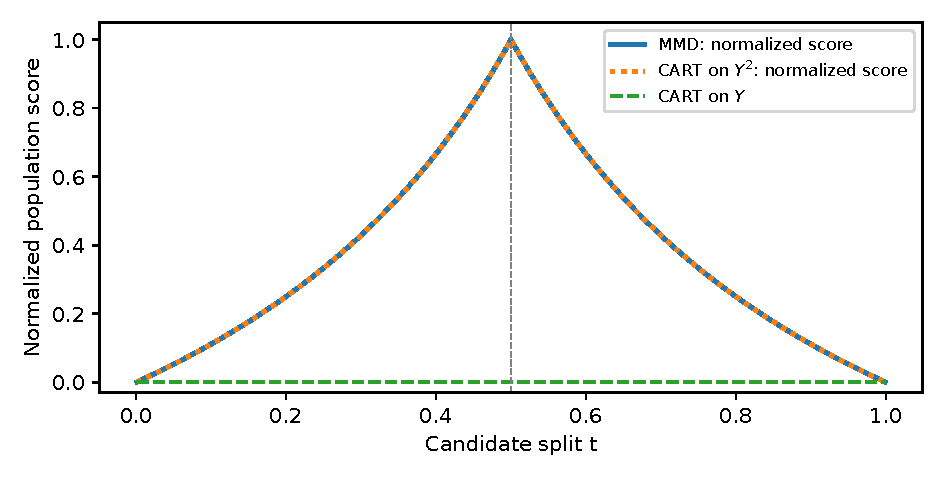
\includegraphics[width=0.79\linewidth]{drf_population_scores.pdf}
\caption{Population splitting criteria in the variance-change example. The MMD and CART-on-$Y^2$ curves are scaled by their positive maxima; CART on $Y$ remains zero. MMD and CART on $Y^2$ identify $\theta_0=0.5$; CART on $Y$ has zero population improvement at every candidate split.}
\label{fig:population}
\end{figure}

\begin{remark}[An important mismatch with the asymptotic assumptions]\label{rem:jump}
The mapping $x\mapsto\mu(x)$ in \eqref{eq:model} jumps at $x=1/2$, violating global Lipschitz continuity. Hence \eqref{eq:model} falls outside the smooth conditional-embedding assumptions used for the global consistency and inference results reviewed in Sections~\ref{sec:consistency} and \ref{sec:inference}. Proposition~\ref{prop:ident} follows from a direct population computation independently of those theorems. Section~\ref{sec:smooth} studies smooth variance transitions that do satisfy these assumptions.
\end{remark}

\section{Numerical Study: Root-Split Comparisons and Kernel Sensitivity}\label{sec:simulation}
\subsection{Design and Estimators}
This section assesses how three root-splitting rules identify the change point in \eqref{eq:model}: standard squared-error CART on $Y$; squared-error CART on the transformed response $Y^2$; and exact Gaussian-kernel MMD splitting. The second criterion explicitly targets the variance change, providing a stronger baseline than CART on $Y$ alone. I generate $R=200$ independent datasets at each $n\in\{200,400,800\}$, with seed $6242$. Within each dataset, all three methods use the same observations. The candidate thresholds are midpoints of consecutive ordered covariate observations, with at least $\lceil0.15n\rceil$ observations in each child.

Every method maximizes the balanced score. For the transformed CART baseline this is $n_Ln_R(\overline{Y^2}_L-\overline{Y^2}_R)^2/n_I^2$. MMD uses the biased empirical squared discrepancy, including diagonal terms, evaluated from the exact Gaussian kernel matrix with $h=1$; the practical DRF random-feature approximation is outside the scope of this experiment. Let $\widehat\theta$ denote the maximizing threshold. I report the mean and median of $|\widehat\theta-\theta_0|$, its Monte Carlo standard error (MCSE), and the fraction within $0.1$ of the true change point.

\subsection{Root-Split Results}\label{sec:results}
\begin{table}[htbp]
\centering\small
\caption{Change-point error across 200 independent replications. MCSE is the Monte Carlo standard error of the \emph{mean absolute error}. All methods use the same datasets at each sample size.}
\label{tab:simulation}
\begin{tabular}{@{}rlrrrr@{}}
\toprule
$n$ & Split rule & Mean abs. error & MCSE & Median abs. error & Within $0.1$ \\
\midrule
200 & CART on $Y$ & 0.20720 & 0.00750 & 0.22486 & 0.205 \\
200 & CART on $Y^2$ & 0.04757 & 0.00501 & 0.01983 & 0.870 \\
200 & MMD ($h=1$) & 0.03692 & 0.00374 & 0.01655 & 0.905 \\
400 & CART on $Y$ & 0.21557 & 0.00736 & 0.22479 & 0.180 \\
400 & CART on $Y^2$ & 0.01957 & 0.00196 & 0.00923 & 0.975 \\
400 & MMD ($h=1$) & 0.01402 & 0.00117 & 0.00776 & 1.000 \\
800 & CART on $Y$ & 0.22108 & 0.00761 & 0.24788 & 0.185 \\
800 & CART on $Y^2$ & 0.00848 & 0.00095 & 0.00410 & 0.995 \\
800 & MMD ($h=1$) & 0.00634 & 0.00050 & 0.00394 & 1.000 \\
\bottomrule
\end{tabular}
\end{table}

Table~\ref{tab:simulation} reports the errors. The mean-oriented CART root split does not improve as $n$ increases, consistent with its flat population objective. Its errors are not merely diffuse, however: Figure~\ref{fig:boxplots} shows that its splits are pulled into the high-variance regime, with median $0.73$ and $84\%$ of splits above $1/2$ at $n=800$. A heuristic explains this. Because the conditional mean is zero everywhere, the balanced CART score at a split with left fraction $t$ has expectation $n^{-1}[(1-t)v_L(t)+t\,v_R(t)]$, where $v_L,v_R$ are the average conditional variances in the two children. In model \eqref{eq:model} this increases from about $1.27/n$ at $t=0.15$ to about $3.74/n$ at $t=0.85$, so the noise maximizer drifts towards the high-variance side.

Both variance-sensitive criteria produce much smaller errors, which decrease with $n$. MMD is more accurate than CART on $Y^2$ at every sample size. The paired mean differences (MMD minus CART on $Y^2$), computed from within-dataset differences, are $-0.01065$ ($\pm0.00519$), $-0.00555$ ($\pm0.00184$), and $-0.00215$ ($\pm0.00091$) at $n=200,400,800$, i.e., about $2$--$3$ MCSEs below zero. At $n=800$, the mean absolute errors are $0.0063$ for MMD and $0.0085$ for CART on $Y^2$. A plausible explanation is robustness: $Y^2$ is a scaled $\chi^2_1$ variable with heavy right tail, so a few large squared responses can move the CART-on-$Y^2$ split, whereas the bounded Gaussian kernel limits the influence of any single observation.
\begin{figure}[htbp]
\centering
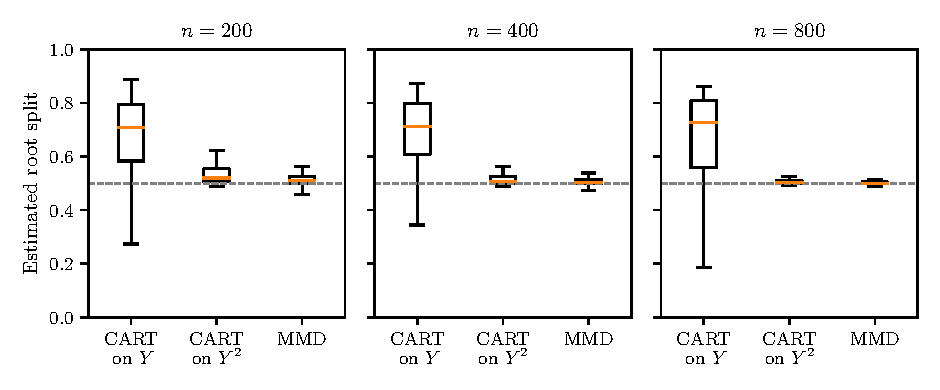
\includegraphics[width=\linewidth]{drf_split_boxplots.pdf}
\caption{Estimated root split across 200 replications at each sample size. Dashed horizontal lines mark the true threshold $\theta_0=0.5$. Boxes depict the median and interquartile range (IQR); whiskers follow the default $1.5\,\mathrm{IQR}$ convention and omit plotted outliers.}
\label{fig:boxplots}
\end{figure}

\subsection{Sensitivity to the Gaussian Kernel Bandwidth}
In a separate simulation with $n=400$, $R=120$, and seed $6243$, I compare exact MMD splitting using $h\in\{0.25,0.5,1,2,4\}$. All bandwidths are evaluated on the same 120 datasets; the bandwidth is fixed in advance for each comparison. The results are summarized in Table~\ref{tab:bandwidth} and Figure~\ref{fig:bandwidth}.
\begin{table}[htbp]
\centering\small
\caption{Bandwidth sensitivity for exact Gaussian MMD root splitting ($n=400$, 120 replications). MCSE quantifies simulation uncertainty for the mean absolute error.}
\label{tab:bandwidth}
\begin{tabular}{@{}rrrrr@{}}
\toprule
$h$ & Mean abs. error & MCSE & Median abs. error & Within $0.1$ \\
\midrule
0.25 & 0.01829 & 0.00248 & 0.00783 & 0.958 \\
0.50 & 0.01493 & 0.00181 & 0.00704 & 0.983 \\
1.00 & 0.01345 & 0.00177 & 0.00652 & 0.983 \\
2.00 & 0.01233 & 0.00162 & 0.00538 & 1.000 \\
4.00 & 0.03165 & 0.00532 & 0.00740 & 0.908 \\
\bottomrule
\end{tabular}
\end{table}
\begin{figure}[htbp]
\centering
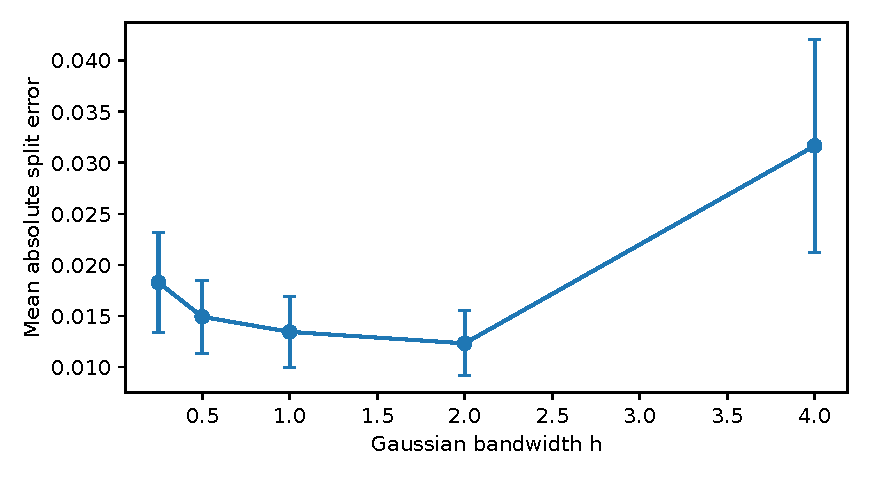
\includegraphics[width=0.77\linewidth]{drf_bandwidth_sensitivity.pdf}
\caption{Mean absolute split error by Gaussian kernel bandwidth. Error bars are $\pm1.96$ Monte Carlo standard errors of the estimated means and represent simulation precision.}
\label{fig:bandwidth}
\end{figure}

Within this grid, $h=2$ has the smallest observed mean absolute error ($0.01233$), followed closely by $h=1$ ($0.01345$). For the matched datasets, the mean error difference between $h=2$ and $h=1$ is $-0.00112$ with paired MCSE $0.00160$. The error rises at $h=4$. The ranking is specific to this variance-change model and finite sample sizes; the paired comparison does not establish a clear advantage of $h=2$ over $h=1$.

\subsection{Interpretation and Limitations}
The analysis isolates the effect of the splitting target. A second-moment transformation recovers the variance signal when one knows to look for it; MMD recovers it without being told, and here does so slightly more accurately. This experiment uses one covariate, scalar Gaussian responses, and a single split, and Remark~\ref{rem:jump} applies. Section~\ref{sec:fullforest} extends the evaluation to complete forests and further distributional alternatives.


\section{Full-Forest Evaluation Across Distributional Alternatives}\label{sec:fullforest}
\subsection{Research Question and Experimental Models}
The preceding experiments isolate a single root split. This section examines whether distribution-oriented tree partitions improve the estimated \emph{conditional law} after aggregation over many trees. The evaluation considers four data-generating mechanisms. In every setting $X=(X^{(1)},X^{(2)},X^{(3)})\sim U([0,1]^3)$; the superscript indexes covariate coordinates, with $X_i^{(j)}$ denoting coordinate $j$ of training observation $i$. The response distribution depends on the first coordinate through $G(x)=\1\{x^{(1)}>1/2\}$, and $X^{(2)},X^{(3)}$ are independent nuisance covariates. Here $t_3$ denotes a Student $t$ random variable with three degrees of freedom, $a=0.95$ specifies the separation in the Gaussian mixture, and $N_2(0,\Sigma)$ denotes a bivariate normal law with covariance matrix $\Sigma$. The four conditional response laws are
\begin{align}
\text{Variance:}\quad & Y\mid X=x\sim
 \begin{cases}N(0,1),&G(x)=0,\\N(0,4),&G(x)=1;\end{cases}\label{eq:ffvariance}\\[2pt]
\text{Tail shape:}\quad & Y\mid X=x\sim
 \begin{cases}N(0,1),&G(x)=0,\\t_3/\sqrt{3},&G(x)=1;\end{cases}\label{eq:fftail}\\[2pt]
\text{Bimodality:}\quad &Y\mid X=x\sim
 \begin{cases}N(0,1),&G(x)=0,\\ \frac12N(-a,1-a^2)+\frac12N(a,1-a^2),&G(x)=1.\end{cases}\label{eq:ffmix}
\end{align}
The variable $t_3/\sqrt{3}$ has unit variance, and both distributions in \eqref{eq:ffmix} have mean zero and variance one. Finally, for $Y\in\R^2$,
\begin{equation}\label{eq:ffdep}
 \begin{aligned}
 \text{Dependence:}\qquad Y\mid X=x&\sim N_2(0,\Sigma_{G(x)}),\\
 \Sigma_0&=\begin{pmatrix}1&0.8\\0.8&1\end{pmatrix},\qquad
 \Sigma_1=\begin{pmatrix}1&-0.8\\-0.8&1\end{pmatrix}.
 \end{aligned}
\end{equation}
In the bivariate case, write $Y=(Y^{(1)},Y^{(2)})$, where parenthesized superscripts index the response coordinates. The dependence alternative preserves both marginal response laws. These designs isolate changes in scale, tail shape, modality, and joint dependence; the bimodality design plays the same role as the constant-mean, constant-variance scenario of \cite[Section~4.2]{cevid2022}. All four are step changes at $x^{(1)}=1/2$, so Remark~\ref{rem:jump} applies; Section~\ref{sec:smooth} studies smooth transitions.

The strength of each distributional signal, as seen by the kernel used for splitting, is the between-regime discrepancy $D_h=\MMD_{k_h}^2(P_0,P_1)$ of Proposition~\ref{prop:ident}. I compute it exactly (by quadrature for the Student law): $D_h=0.0942$ (variance), $0.0165$ (tail shape), $0.0221$ (bimodality), and $0.0923$ (dependence, $h=1.4$). By Proposition~\ref{prop:ident}, the population MMD split score is proportional to $D_h$, so the tail-shape and bimodality changes give four to six times less population signal than the variance and dependence changes.

\subsection{Forest Construction and Distributional Predictions}
I compare two finite, $B=180$-tree bootstrap ensembles with identical training covariates, bootstrap randomization, and tree hyperparameters. The \emph{mean-CART forest} splits using the original scalar or multivariate response $Y$. Its terminal-leaf weights define a weighted empirical conditional law, as in quantile regression forests. The second model, termed the \emph{RFF--MMD forest}, constructs a shared feature map from $M=48$ independent Gaussian Fourier frequencies:
\begin{equation}\label{eq:fffeatures}
 \psi_M(y)=\frac1{\sqrt M}\bigl(
 \cos(\omega_1^\top y),\ldots,\cos(\omega_M^\top y),
 \sin(\omega_1^\top y),\ldots,\sin(\omega_M^\top y)\bigr),\qquad
 \omega_j\sim N(0,h^{-2}I_d).
\end{equation}
For a candidate split with child index sets $I_L,I_R$, define the empirical feature means $\overline\psi_{M,L}=n_L^{-1}\sum_{i\in I_L}\psi_M(Y_i)$ and $\overline\psi_{M,R}=n_R^{-1}\sum_{i\in I_R}\psi_M(Y_i)$. Multioutput squared-error CART is fitted to $\psi_M(Y)$, so its empirical variance reduction for a prospective split is proportional to
\[
 \frac{n_Ln_R}{n_I^2}\bigl\|\overline\psi_{M,L}-\overline\psi_{M,R}\bigr\|_2^2,
\]
which approximates the MMD score in \eqref{eq:drfscore}. This provides a reproducible implementation of the distribution-sensitive forest splitting principle using standard tree software. The Fourier features are fixed throughout each fitted forest; the original DRF algorithm resamples them at every node. Both forests use ordinary bootstrap trees with no sample-splitting honesty. Consequently, the experiment evaluates an \emph{RFF approximation to MMD-splitting forests}, and the asymptotic inference theory of N\"af et al.\ \cite{naf2023} is outside its scope.

For a query $x$, let $N_{bi}(x)$ be the number of bootstrap occurrences of training observation $i$ in the leaf containing $x$ for tree $b$. The denominator $\sum_{j=1}^nN_{bj}(x)$ counts bootstrap observations in that leaf, including repeated occurrences. Both ensembles form valid distributional weights
\begin{equation}\label{eq:ffweights}
 \widehat w_{i,B}(x)=\frac1B\sum_{b=1}^B
 \frac{N_{bi}(x)}{\sum_{j=1}^nN_{bj}(x)},\qquad
 \widehat P_{x,B}=\sum_{i=1}^n\widehat w_{i,B}(x)\delta_{Y_i}.
\end{equation}
Bootstrap multiplicities are counted explicitly in every leaf. Each repetition uses $n=650$ training pairs, $360$ independent query--response pairs, and random forest parameters \texttt{max\_features=2}, \texttt{min\_samples\_leaf=12}, and \texttt{bootstrap=True}. The Gaussian bandwidth is $h=1$ for scalar responses and $h=1.4$ for the bivariate dependence setting. All parameters were fixed for this comparison. There are $R=25$ independent repetitions per setting, using matched datasets for the two estimators.

\subsection{Evaluation Metrics}
Let $X_1^{\mathrm{test}},\ldots,X_{n_{\mathrm{test}}}^{\mathrm{test}}$ be independent test covariate vectors, where $n_{\mathrm{test}}=360$ in each replication. The model $P_{X_j^{\mathrm{test}}}$ is the true conditional response law at test covariate $X_j^{\mathrm{test}}$, and $\widehat P_{X_j^{\mathrm{test}},B}$ is its forest estimate. The primary distributional metric is squared MMD to this known true conditional law:
\begin{equation}\label{eq:ffmmdrisk}
 \widehat{\mathcal R}_{\mathrm{MMD}}
 =\frac1{n_{\mathrm{test}}}\sum_{j=1}^{n_{\mathrm{test}}}
  \MMD_{k_h}^2\bigl(\widehat P_{X_j^{\mathrm{test}},B},P_{X_j^{\mathrm{test}}}\bigr).
\end{equation}
This quantity is evaluated using exact Gaussian convolution formulas for normal laws and Gaussian mixtures; the Student alternative uses $4096$-point deterministic midpoint quantile quadrature. Both the empirical-law/Student cross term and the Student/Student kernel expectation use this rule. With the two fitted estimators fixed at the first tail-shape replication, increasing the grid from $4096$ to $8192$ changes the mean conditional squared MMD by at most $3.26\times10^{-8}$ and any individual query score by at most $6.30\times10^{-8}$. These changes are much smaller than the reported Monte Carlo errors. This is a convergence diagnostic for that replication, rather than a uniform error bound over all fitted estimators. The evaluation kernel $k_h$ is the same Gaussian family used for the Fourier features, but the score uses the exact Gaussian kernel, independently of the feature approximation.

As a complementary metric, let $\Lambda$ denote a specified real-valued functional on probability measures. The mean absolute error of its plug-in forest estimate is
\begin{equation}\label{eq:fffunctional}
  \widehat{\mathcal R}_{\Lambda}=\frac1{n_{\mathrm{test}}}
 \sum_{j=1}^{n_{\mathrm{test}}}
  \left|\Lambda(\widehat P_{X_j^{\mathrm{test}},B})-\Lambda(P_{X_j^{\mathrm{test}}})\right|.
\end{equation}
The chosen functionals $\Lambda$ are conditional variance for \eqref{eq:ffvariance}, $P(|Y|\le1\mid X=x)$ for \eqref{eq:fftail}, $P(|Y|\le0.5\mid X=x)$ for \eqref{eq:ffmix}, and conditional covariance $\operatorname{Cov}(Y^{(1)},Y^{(2)}\mid X=x)$ for \eqref{eq:ffdep}. The tail-shape target measures probability in the central region, which changes along with the tails. A held-out Gaussian-kernel score is also recorded in the saved results; it is not reported here because its expectation equals the conditional MMD risk plus a constant that depends only on the true law.

Monte Carlo standard errors (MCSEs) use the $R=25$ independent datasets as the replication units. For each metric, let $d_r$ be the error of RFF--MMD minus the error of mean-CART on the same dataset $r$. I report
\begin{equation}\label{eq:pairedmcse}
 \overline d=\frac1R\sum_{r=1}^R d_r,\qquad
 \operatorname{MCSE}(\overline d)=
 \sqrt{\frac{1}{R(R-1)}\sum_{r=1}^R(d_r-\overline d)^2}.
\end{equation}
A negative contrast favors RFF--MMD. The test covariates and individual trees are not independent Monte Carlo replications. These MCSEs describe simulation precision, rather than uncertainty intervals for a conditional law estimated from one training dataset.

\subsection{Results: Conditional Distribution and Functional Accuracy}
\begin{table}[htbp]
\centering\small
\caption{Full-forest distributional estimation error: mean $\pm$ MCSE across 25 independent datasets. Smaller conditional MMD$^2$ indicates a more accurate estimate of $P_x$. The Student alternative uses deterministic quadrature.}
\label{tab:ffmmd}
\begin{tabular}{@{}lcc@{}}
\toprule
Scenario & Mean-CART forest & RFF--MMD forest \\
\midrule
Variance change & $0.01509\pm 0.00041$ & $0.01599\pm 0.00044$ \\
Tail-shape change & $0.01003\pm 0.00033$ & $0.01128\pm 0.00037$ \\
Matched-moment bimodality & $0.01416\pm 0.00050$ & $0.01481\pm 0.00047$ \\
Dependence change & $0.01348\pm 0.00029$ & $0.01290\pm 0.00038$ \\
\bottomrule
\end{tabular}
\end{table}

\begin{table}[htbp]
\centering\small
\caption{Full-forest mean absolute errors for scenario-specific conditional functionals, mean $\pm$ MCSE. Functional scales differ across scenarios.}
\label{tab:fffunction}
\begin{tabular}{@{}lcc@{}}
\toprule
Scenario & Mean-CART forest & RFF--MMD forest \\
\midrule
Variance change & $0.58593\pm 0.01601$ & $0.44033\pm 0.01327$ \\
Tail-shape change & $0.04475\pm 0.00134$ & $0.05227\pm 0.00162$ \\
Matched-moment bimodality & $0.07021\pm 0.00181$ & $0.04992\pm 0.00225$ \\
Dependence change & $0.28388\pm 0.00564$ & $0.15174\pm 0.00351$ \\
\bottomrule
\end{tabular}
\end{table}

\begin{figure}[htbp]
\centering
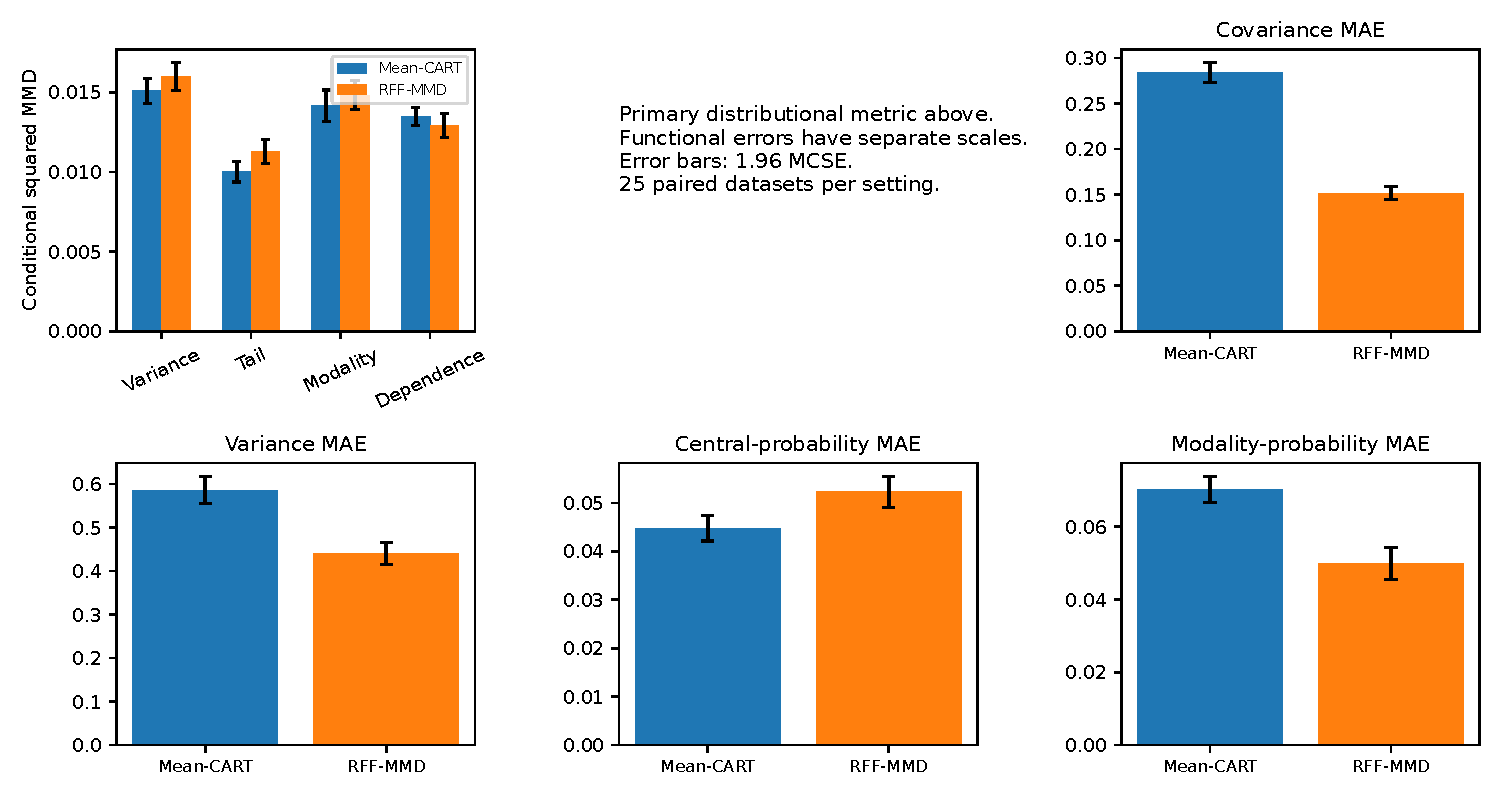
\includegraphics[width=\linewidth]{drf_full_forest_scores.pdf}
\caption{Full-forest comparison in four settings, 25 paired datasets each. Left: conditional squared MMD to the true law (primary metric). Right: mean absolute error of the scenario-specific functional, on its own scale. Error bars equal $1.96$ individual-method MCSEs; paired comparisons appear in Table~\ref{tab:ffpaired}.}
\label{fig:fullforest}
\end{figure}

\begin{table}[htbp]
\centering\small
\caption{Paired error contrasts, RFF--MMD minus mean-CART: mean difference $\pm$ paired MCSE over 25 independent datasets. Negative values favor RFF--MMD. Functional units differ across scenarios.}
\label{tab:ffpaired}
\begin{tabular}{@{}lcc@{}}
\toprule
Scenario & Conditional MMD$^2$ difference & Functional MAE difference \\
\midrule
Variance change & $0.00091\pm 0.00037$ & $-0.14560\pm 0.01838$ \\
Tail-shape change & $0.00126\pm 0.00022$ & $0.00752\pm 0.00103$ \\
Matched-moment bimodality & $0.00065\pm 0.00028$ & $-0.02029\pm 0.00208$ \\
Dependence change & $-0.00058\pm 0.00018$ & $-0.13214\pm 0.00635$ \\
\bottomrule
\end{tabular}
\end{table}

The primary distributional metric in Table~\ref{tab:ffmmd} favors mean-CART for variance, tail shape, and bimodality; RFF--MMD has a smaller error for dependence. The functional results in Table~\ref{tab:fffunction} differ: RFF--MMD yields smaller errors for conditional variance, the modality-sensitive probability, and conditional covariance. For covariance, mean absolute error decreases from $0.2839$ to $0.1517$. The central probability in the tail-shape setting favors mean-CART ($0.0447$ compared with $0.0523$). Table~\ref{tab:ffpaired} quantifies the matched comparisons directly, using the dataset as the unit of replication. Figure~\ref{fig:fullforest} displays the individual-method means.

\subsection{Explaining the Rankings: A Bias--Remainder Decomposition}\label{sec:decomposition}
Why does a forest designed to track distributional change estimate three of four conditional laws less accurately in MMD, while estimating the targeted functionals more accurately? Because the true conditional laws are known, the conditional MMD risk can be split exactly. Writing $\mu(X_i)$ for the true embedding at a training covariate,
\begin{equation}\label{eq:decomp}
 \MMD_{k_h}^2\bigl(\widehat P_{x,B},P_x\bigr)
 =\underbrace{\Bigl\|\sum_i\widehat w_{i,B}(x)\mu(X_i)-\mu(x)\Bigr\|_{\calH}^2}_{\text{localization bias}}
 +\underbrace{\mathcal R(x)}_{\text{remainder}},
\end{equation}
where $\mathcal R(x)$ collects the noise $\|\sum_i\widehat w_{i,B}(x)\{k_h(Y_i,\cdot)-\mu(X_i)\}\|_{\calH}^2$ and a cross term. In the step designs, $\mu(X_i)$ equals $\mu_0$ or $\mu_1$, so $\sum_i\widehat w_{i,B}(x)\mu(X_i)=W_0\mu_0+W_1\mu_1$ and, by the argument of Proposition~\ref{prop:ident}, the bias equals $m(x)^2D_h$. Here $m(x)$ is the total weight the forest places on training points from the opposite regime. If the weights did not depend on the training responses, as for honest trees, the cross term would have mean zero and the noise would have mean equal to the \emph{noise proxy} $\sum_i\widehat w_{i,B}(x)^2\{1-\|\mu(X_i)\|_{\calH}^2\}$, using $k_h(y,y)=1$. Its size is governed by the effective sample size $n_{\mathrm{eff}}(x)=1/\sum_i\widehat w_{i,B}(x)^2$. I call $\mathcal R(x)$ minus the noise proxy the \emph{excess}; it measures the effect of using the same responses both to choose splits and to populate leaves. Table~\ref{tab:decomp} and Figure~\ref{fig:decomp} report these quantities, averaged over test points and datasets.

\begin{table}[htbp]
\centering\footnotesize
\caption{Decomposition \eqref{eq:decomp} of the conditional MMD$^2$ risk; means over 25 datasets. $D_h$, bias, remainder, noise proxy, and excess (remainder minus noise proxy) are multiplied by $10^3$. $m$ is the mean weight on opposite-regime training points and $n_{\mathrm{eff}}$ the mean effective sample size.}
\label{tab:decomp}
\begin{tabular}{@{}lrlrrrrrr@{}}
\toprule
Scenario & $10^3D_h$ & Forest & $m$ & Bias & Remainder & Noise proxy & Excess & $n_{\mathrm{eff}}$ \\
\midrule
\multirow{2}{*}{Variance} & \multirow{2}{*}{94.2} & Mean-CART & 0.160 & 3.63 & 11.46 & 5.65 & 5.80 & 99.0 \\
 &  & RFF--MMD & 0.039 & 0.67 & 15.32 & 6.20 & 9.12 & 89.4 \\
\addlinespace
\multirow{2}{*}{Tail shape} & \multirow{2}{*}{16.5} & Mean-CART & 0.207 & 0.92 & 9.10 & 3.74 & 5.37 & 102.8 \\
 &  & RFF--MMD & 0.109 & 0.39 & 10.89 & 3.99 & 6.90 & 96.1 \\
\addlinespace
\multirow{2}{*}{Bimodality} & \multirow{2}{*}{22.1} & Mean-CART & 0.207 & 1.23 & 12.93 & 4.28 & 8.65 & 103.3 \\
 &  & RFF--MMD & 0.093 & 0.41 & 14.41 & 4.63 & 9.78 & 95.5 \\
\addlinespace
\multirow{2}{*}{Dependence} & \multirow{2}{*}{92.3} & Mean-CART & 0.154 & 3.35 & 10.13 & 4.68 & 5.45 & 100.4 \\
 &  & RFF--MMD & 0.017 & 0.22 & 12.68 & 5.39 & 7.29 & 86.7 \\
\bottomrule
\end{tabular}
\end{table}

\begin{figure}[htbp]
\centering
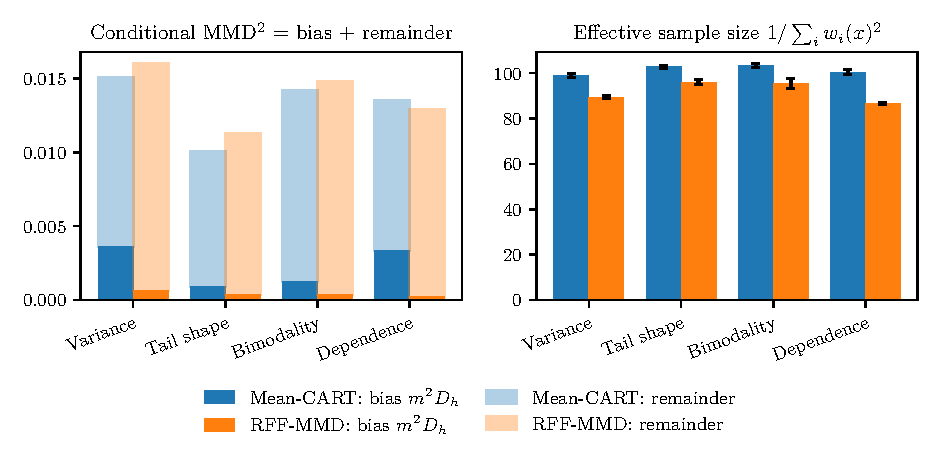
\includegraphics[width=\linewidth]{drf_full_forest_decomposition.pdf}
\caption{Left: conditional MMD$^2$ split into localization bias $m^2D_h$ (solid) and remainder (hatched). Right: mean effective sample size of the forest weights, with $\pm1.96$ MCSE.}
\label{fig:decomp}
\end{figure}

The decomposition resolves the apparent contradiction. RFF--MMD localizes far better: the weight on the wrong regime falls from $0.160$ to $0.039$ in the variance setting and from $0.154$ to $0.017$ in the dependence setting, and the paired change in bias ($\times10^3$) is $-2.95\pm0.18$ and $-3.13\pm0.12$, respectively. This is why the variance, bimodality-probability, and covariance functionals improve: the regimes differ substantially in these targets, so placing less weight on the wrong regime pays off. However, in these two settings the remainder grows by $3.86\pm0.33$ and $2.56\pm0.18$. Only in the dependence setting does the bias reduction exceed the growth of the remainder, which is exactly the one setting where RFF--MMD wins on MMD$^2$. In the tail-shape and bimodality settings, $D_h$ is small, so even perfect localization could save at most about $10^{-3}$, and the larger remainder dominates. The same remainder growth explains the one functional that does not improve, the tail-shape central probability: RFF--MMD is worse there even though it roughly halves $m$ (from $0.207$ to $0.109$), because for this target the extra variability outweighs the smaller localization gain.

The growth of the remainder is only partly due to more concentrated weights. RFF--MMD does have smaller effective sample sizes ($89$ against $99$ in the variance setting), but the noise proxy rises by less than $10^{-3}$ in every setting. Most of the increase is in the excess, which is already as large as or larger than the noise proxy for mean-CART, and larger still for RFF--MMD. The likely mechanism is that a non-honest tree chooses splits that make the empirical response distributions within its leaves as homogeneous as possible. Those same responses then populate the leaves, so the weighted empirical law understates the true conditional variability. The MMD criterion optimizes this homogeneity directly, so the effect is stronger. This dependence between the weights and the leaf responses is exactly what the honesty condition of the assigned papers (Section~\ref{sec:consistency}; assumption (F1) of N\"af et al.) is designed to remove, and it suggests that an honest implementation would retain RFF--MMD's localization gain while removing much of its remainder penalty.

\subsection{Smooth Variance Transitions}\label{sec:smooth}
All preceding designs violate the Lipschitz condition of the theory. To study designs that satisfy it, I replace the variance step by
\begin{equation}\label{eq:smoothvariance}
 Y\mid X=x\sim N\bigl(0,v_\varepsilon(x^{(1)})\bigr),\qquad
 v_\varepsilon(t)=1+3\bigl[1+\exp\{-(t-1/2)/\varepsilon\}\bigr]^{-1},\quad \varepsilon>0,
\end{equation}
with the step change as the limit $\varepsilon\to0$. Here $\varepsilon$ controls the width of the transition; for every $\varepsilon>0$, $x\mapsto\mu(x)$ is Lipschitz because $v_\varepsilon$ is Lipschitz and $\|\mu_{N(0,a)}-\mu_{N(0,b)}\|_{\calH}$ is Lipschitz in the variances on $[1,4]$. All other settings match the variance scenario above ($h=1$, $25$ paired datasets per $\varepsilon$, new seeds). Because the datasets are new, the step row of Table~\ref{tab:smooth} differs from the variance row of Table~\ref{tab:ffmmd} by Monte Carlo error ($14.23$ versus $15.09\times10^{-3}$ for mean-CART). The conditional MMD$^2$ and its bias term remain exact: for Gaussian laws, $\ip{\mu_{N(0,a)}}{\mu_{N(0,b)}}_{\calH}=(1+(a+b)/h^2)^{-1/2}$, so the bias $\|\sum_i\widehat w_{i,B}(x)\mu(X_i)-\mu(x)\|_{\calH}^2$ is a quadratic form in the weights.

\begin{table}[htbp]
\centering\footnotesize
\caption{Smooth variance transitions: mean $\pm$ MCSE over 25 datasets per width $\varepsilon$; paired differences are RFF--MMD minus mean-CART (negative favors RFF--MMD).}
\label{tab:smooth}
\begin{tabular}{@{}lcccccc@{}}
\toprule
& \multicolumn{3}{c}{Conditional MMD$^2$ ($\times10^3$)} & \multicolumn{3}{c}{Conditional-variance MAE} \\
\cmidrule(lr){2-4}\cmidrule(l){5-7}
$\varepsilon$ & Mean-CART & RFF--MMD & Paired diff. & Mean-CART & RFF--MMD & Paired diff. \\
\midrule
step & $14.23\pm0.30$ & $15.71\pm0.39$ & $1.48\pm0.34$ & $0.584\pm0.014$ & $0.402\pm0.011$ & $-0.182\pm0.014$ \\
0.025 & $14.12\pm0.24$ & $16.50\pm0.48$ & $2.38\pm0.41$ & $0.539\pm0.018$ & $0.418\pm0.012$ & $-0.121\pm0.018$ \\
0.05 & $13.05\pm0.44$ & $14.85\pm0.43$ & $1.81\pm0.25$ & $0.499\pm0.015$ & $0.400\pm0.011$ & $-0.099\pm0.016$ \\
0.1 & $13.52\pm0.37$ & $15.97\pm0.48$ & $2.44\pm0.32$ & $0.424\pm0.012$ & $0.404\pm0.011$ & $-0.019\pm0.013$ \\
0.2 & $12.82\pm0.45$ & $15.25\pm0.38$ & $2.44\pm0.31$ & $0.380\pm0.010$ & $0.411\pm0.011$ & $0.031\pm0.009$ \\
\bottomrule
\end{tabular}
\end{table}

\begin{figure}[htbp]
\centering
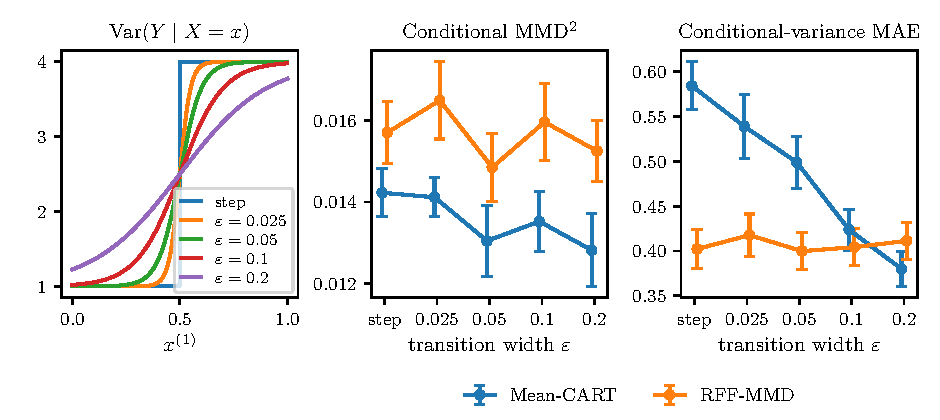
\includegraphics[width=\linewidth]{drf_smooth_transition.pdf}
\caption{Smooth variance transitions. Left: conditional variance functions $v_\varepsilon$. Middle and right: conditional MMD$^2$ and conditional-variance MAE against transition width, with $\pm1.96$ MCSE error bars.}
\label{fig:smooth}
\end{figure}

Table~\ref{tab:smooth} and Figure~\ref{fig:smooth} show that RFF--MMD has the larger conditional MMD$^2$ at every width. Its advantage for conditional variance shrinks steadily as the transition widens. The paired difference is $-0.182\pm0.014$ for the step, $-0.019\pm0.013$ at $\varepsilon=0.1$, and $0.031\pm0.009$ at $\varepsilon=0.2$, where mean-CART is better. The decomposition again explains this. As the transition widens, neighboring conditional laws become more similar, so mixing them costs less: the bias ($\times10^3$) of mean-CART falls from $3.48$ for the step to $0.91$ at $\varepsilon=0.2$, while that of RFF--MMD stays between $0.30$ and $0.56$. Distribution-sensitive localization is therefore most valuable for abrupt changes, which is also where the theory does not apply. Under the smoothness assumed by the theory, its benefit in this non-honest implementation is outweighed by its remainder penalty.

\section{Discussion and Possible Research Directions}\label{sec:discussion}
The assigned papers provide a coherent framework for conditional distribution learning and its inference: MMD-based partitions define a conditional kernel embedding estimator, and half-sampling approximates its sampling distribution under regularity assumptions. The change-point result of Section~\ref{sec:original} shows exactly what a balanced MMD split targets when the conditional mean carries no signal, and the root-split simulations show that this population advantage is realized in finite samples, slightly more accurately than with a hand-chosen $Y^2$ transformation. The full-forest studies suggest a more nuanced picture. Distribution-sensitive splitting does localize much better, but in a non-honest forest this gain is offset by an adaptivity penalty in the remainder of the risk. The net effect depends on the size of the between-regime discrepancy and on how abruptly the conditional law changes.

\paragraph{Honesty.}
The most direct follow-up is to refit both forests with honest trees, using one half of each subsample for splits and the other half for leaf weights, as the honesty condition of both assigned papers requires. The decomposition \eqref{eq:decomp} predicts that honesty should remove most of the excess term for both methods while preserving RFF--MMD's lower misassignment $m$. If so, the MMD$^2$ ranking could reverse in the variance setting, where the bias gap is largest. Honesty also makes the noise proxy an unbiased estimate of the noise term, so the decomposition would become an exact bias--variance decomposition in expectation. The simplest way to also satisfy the Honesty$^*$ condition of Section~\ref{sec:prooffix} is to build each leaf from the structure half alone, without adjusting it to the estimation half, at the cost of controlling leaf sizes on the estimation half only approximately. The honest comparisons of Koemen \cite{koemen2026}, in which honesty can matter as much as the splitting criterion, suggest that this experiment could change the conclusions of Section~\ref{sec:fullforest}. The official DRF package \cite{cevid2022} implements honest trees and, by fitting trees in groups that share a half-sample, the uncertainty estimates of \cite{naf2023}, which would allow coverage to be checked on the smooth designs of Section~\ref{sec:smooth}, where the theory applies.

\paragraph{Kernel choice and forest construction.}
The root-split bandwidth study shows sensitivity to kernel scale, and Section~\ref{sec:fullforest} shows that the attainable gain from localization scales with $D_h$, which itself depends on $h$. A natural extension would choose $h$ to maximize $D_h$ over plausible alternatives, or aggregate over several bandwidths, and vary the number of Fourier frequencies, the minimum leaf size, and resampling of frequencies at each node, selecting hyperparameters on a separate validation sample.

\paragraph{Tails.}
The tail-shape central probability is the one targeted functional that RFF--MMD does not improve, and any weighted empirical law \eqref{eq:weightedlaw} puts no mass beyond the observed responses. A natural combination is to keep MMD splitting for the body of the distribution and, as in extremal random forests \cite{gnecco2024}, fit a generalized Pareto tail by local likelihood with the DRF weights. The Student design of Section~\ref{sec:fullforest} would show whether this improves upper-tail probabilities without losing the localization gain of MMD splitting.

\paragraph{Smoothness.}
The smooth-transition results suggest that the benefit of distribution-sensitive splitting is greatest for abrupt changes, outside the Lipschitz setting of the consistency and inference theorems. A rate analysis that interpolates between the two regimes, for example with a transition width $\varepsilon_n\to0$, could clarify when MMD splitting attains a faster rate than mean splitting.

\section{Conclusion}\label{sec:conclusion}
The assigned papers establish a general approach to estimating conditional response distributions with forests and to quantifying sampling uncertainty in the associated RKHS. My population analysis proves change-point identification by balanced MMD splitting under piecewise-constant conditional laws, and root-split simulations confirm that MMD locates a pure variance change more accurately than both mean-CART and CART on $Y^2$. In complete forests, an RFF approximation to MMD splitting improves three of four targeted functionals but has larger conditional MMD$^2$ in three of four settings. An exact bias--remainder decomposition shows why: RFF--MMD sharply reduces the weight on the wrong regime, but non-honest leaves inflate the remainder by more than the bias falls, except in the dependence setting. In smooth transitions, which satisfy the theory's Lipschitz assumption, the variance advantage of RFF--MMD disappears. These findings identify honesty, kernel tuning, and the smoothness of the covariate-to-distribution map as the key factors in whether distribution-sensitive splitting pays off. The follow-up literature has broadened the scope of DRF and repaired one step of its inference theory, but faster rates, guarantees without honesty, and inference uniform in $x$ remain open.

\appendix
\section{Derivation of the Hilbert-Space Splitting Identity}\label{app:anova}
For $i$ in a parent node index set $I$, define $z_i=\varphi(Y_i)\in\calH$. For any nonempty node index set $J$, write $\overline z_J=|J|^{-1}\sum_{i\in J}z_i$, abbreviating $\overline z_{I_L}$ and $\overline z_{I_R}$ as $\overline z_L$ and $\overline z_R$, and let $a\in\calH$ be arbitrary. The Hilbert-space decomposition
\[
 \sum_{i\in J}\norm{z_i-a}_{\calH}^2
 =\sum_{i\in J}\norm{z_i-\overline z_J}_{\calH}^2
  +|J|\norm{\overline z_J-a}_{\calH}^2
\]
holds because $\sum_{i\in J}(z_i-\overline z_J)=0$. Apply this separately to $J=I_L$ and $J=I_R$ with $a=\overline z_I$ and divide by $n_I$:
\[
 \widehat V_I=\frac{n_L}{n_I}\widehat V_L+\frac{n_R}{n_I}\widehat V_R
 +\frac{n_L}{n_I}\norm{\overline z_L-\overline z_I}_{\calH}^2
 +\frac{n_R}{n_I}\norm{\overline z_R-\overline z_I}_{\calH}^2.
\]
Because $\overline z_I=(n_L/n_I)\overline z_L+(n_R/n_I)\overline z_R$, the last two terms add to
\[
 \frac{n_Ln_R}{n_I^2}\norm{\overline z_L-\overline z_R}_{\calH}^2.
\]
The two sample embeddings are $\overline z_L=\mu_{\widehat P_L}$ and $\overline z_R=\mu_{\widehat P_R}$, so their squared difference is the empirical squared MMD. This proves \eqref{eq:anova}.

\begin{thebibliography}{99}
\bibitem{athey2019}
S. Athey, J. Tibshirani, and S. Wager (2019).
Generalized random forests.
\emph{The Annals of Statistics}, 47(2), 1148--1178.
\url{https://doi.org/10.1214/18-AOS1709}.

\bibitem{benard2024}
C. B\'enard, J. N\"af, and J. Josse (2024).
MMD-based variable importance for distributional random forest.
In \emph{Proceedings of the 27th International Conference on Artificial Intelligence and Statistics}, PMLR 238, 1324--1332.
\url{https://proceedings.mlr.press/v238/benard24a.html}.

\bibitem{breiman2001}
L. Breiman (2001).
Random forests.
\emph{Machine Learning}, 45, 5--32.
\url{https://doi.org/10.1023/A:1010933404324}.

\bibitem{cevid2022}
D. \'{C}evid, L. Michel, J. N\"af, P. B\"uhlmann, and N. Meinshausen (2022).
Distributional random forests: Heterogeneity adjustment and multivariate distributional regression.
\emph{Journal of Machine Learning Research}, 23(333), 1--79.
\url{https://www.jmlr.org/papers/v23/21-0585.html}.

\bibitem{gnecco2024}
N. Gnecco, E. M. Terefe, and S. Engelke (2024).
Extremal random forests.
\emph{Journal of the American Statistical Association}, 119(548), 3059--3072.
\url{https://doi.org/10.1080/01621459.2023.2300522}.

\bibitem{gretton2012}
A. Gretton, K. M. Borgwardt, M. J. Rasch, B. Sch\"olkopf, and A. Smola (2012).
A kernel two-sample test.
\emph{Journal of Machine Learning Research}, 13, 723--773.
\url{https://www.jmlr.org/papers/v13/gretton12a.html}.

\bibitem{zou2025}
Y. Zou, M. Matabuena, and M. R. Kosorok (2025).
Distributional random forests for complex survey designs.
\emph{arXiv preprint} arXiv:2512.08179 (version 3, 2026).
\url{https://arxiv.org/abs/2512.08179}.

\bibitem{jainluedtke2026}
S. Jain and A. Luedtke (2026).
Conditional distributional treatment effects: Doubly robust estimation and testing.
In \emph{Proceedings of the 43rd International Conference on Machine Learning}, PMLR 306, 50417--50473.
\url{https://proceedings.mlr.press/v306/jain26a.html}.

\bibitem{koemen2026}
S. Koemen (2026).
Distributional split criteria for random forests: Extensions, shrinkage, and the robustness of mean splitting.
\emph{arXiv preprint} arXiv:2607.23721.
\url{https://arxiv.org/abs/2607.23721}.

\bibitem{kundulinero2026}
P. Kundu and A. R. Linero (2026).
Conditional distribution estimation for functional responses with random forests.
\emph{arXiv preprint} arXiv:2608.08247.
\url{https://arxiv.org/abs/2608.08247}.

\bibitem{meinshausen2006}
N. Meinshausen (2006).
Quantile regression forests.
\emph{Journal of Machine Learning Research}, 7, 983--999.
\url{https://www.jmlr.org/papers/v7/meinshausen06a.html}.

\bibitem{naf2023}
J. N\"af, C. Emmenegger, P. B\"uhlmann, and N. Meinshausen (2023).
Confidence and uncertainty assessment for distributional random forests.
\emph{Journal of Machine Learning Research}, 24(366), 1--77.
\url{https://www.jmlr.org/papers/v24/23-0185.html}.

\bibitem{naf2024imp}
J. N\"af, E. Scornet, and J. Josse (2024).
What is a good imputation under MAR missingness?
\emph{arXiv preprint} arXiv:2403.19196 (version 5, 2026).
\url{https://arxiv.org/abs/2403.19196}.

\bibitem{nafpark2026}
J. N\"af, J. Park, and H. Susmann (2026).
Causal-DRF: Conditional kernel treatment effect estimation using distributional random forest.
In \emph{Proceedings of the 29th International Conference on Artificial Intelligence and Statistics}, PMLR 300, 1000--1008.
\url{https://proceedings.mlr.press/v300/naf26a.html}.

\bibitem{pospisil2019}
T. Pospisil and A. B. Lee (2019).
(f)RFCDE: Random forests for conditional density estimation and functional data.
\emph{arXiv preprint} arXiv:1906.07177.
\url{https://arxiv.org/abs/1906.07177}.

\bibitem{qiu2024}
R. Qiu, Z. Yu, and R. Zhu (2024).
Random forest weighted local Fr\'echet regression with random objects.
\emph{Journal of Machine Learning Research}, 25(107), 1--69.
\url{https://jmlr.org/papers/v25/23-0811.html}.

\bibitem{wagerathey2018}
S. Wager and S. Athey (2018).
Estimation and inference of heterogeneous treatment effects using random forests.
\emph{Journal of the American Statistical Association}, 113(523), 1228--1242.
\url{https://doi.org/10.1080/01621459.2017.1319839}.
\end{thebibliography}
\end{document}
